\documentclass[oneside]{book}

\setlength{\headheight}{14.49998pt}
\addtolength{\topmargin}{-2.49998pt}

%librerie
% librerie aggiuntive
\usepackage[letterpaper,top=2cm,bottom=2cm,left=3cm,right=3cm,marginparwidth=1.75cm]{geometry} %pacchetto per la geometria della pagina
\usepackage{amsmath} %pacchetto per le formule matematiche
\usepackage{graphicx} %pacchetto per le immagini
\usepackage{float} %pacchetto per il posizionamento delle immagini
\usepackage{wrapfig} %pacchetto per il posizionamento delle immagini
\usepackage[hidelinks]{hyperref} %pacchetto per i link
\usepackage[english,italian]{babel} %pacchetto per la lingua
\usepackage{xpatch} %pacchetto per le patch
\usepackage{fancyhdr} %pacchetto per le intestazioni
\usepackage{xcolor,soul} %pacchetto per l'evidenziazione del testo
\sethlcolor{lightgray} %colore dell'evidenziazione
\pagestyle{fancy} %stile della pagina
\usepackage{listings} %pacchetto per il codice
\usepackage[numbers]{natbib} %pacchetto per la bibliografia
\usepackage{lipsum} %pacchetto per il testo fittizio
\usepackage{subfig,caption} %pacchetto per le figure

\usepackage{helvet} % Load Helvetica font package
\renewcommand{\rmdefault}{phv} % Set the main font to Helvetica

\usepackage[fontsize=12pt]{scrextend} % set font size to 12pt

\newenvironment{abstract}{}{}
\usepackage{abstract} %pacchetto per l'abstract
% abstract in inglese, al fine di cambiarne il titolo
\xpretocmd{\abstract}{\selectlanguage{english}}{}{} 
\xapptocmd{\endabstract}{\selectlanguage{italian}}{}{}

\usepackage[english]{babel}
\usepackage[italian]{babel}

% \usepackage{geometry}

\usepackage[T1]{fontenc}
\usepackage{inconsolata}
\usepackage{color}
\definecolor{bluekeywords}{rgb}{0.13,0.13,1}
\definecolor{greencomments}{rgb}{0,0.5,0}
\definecolor{redstrings}{rgb}{0.9,0,0}
\usepackage{listings}
\lstset{language=[Sharp]C,
  showspaces=false,
  showtabs=false,
  numbers=left,
  breaklines=true,
  showstringspaces=false,
  breakatwhitespace=true,
  escapeinside={*@}{@*},
  commentstyle=\color{greencomments},
  keywordstyle=\color{bluekeywords},
  stringstyle=\color{redstrings},
  basicstyle=\ttfamily,
  postbreak=\mbox{\textcolor{red}{$\hookrightarrow$}\space},
}
\lstdefinelanguage{TypeScript}{
  morekeywords={abstract, as, any, async, await, boolean, break, case, catch, class, console, const, constructor, continue, debugger, declare, default, delete, do, else, enum, export, extends, false, finally, for, from, function, get, if, implements, import, in, infer, instanceof, interface, let, module, new, null, number, object, package, private, protected, public, return, set, static, string, super, switch, this, throw, true, try, type, typeof, var, void, while, with, yield},
  morecomment=[l]{//},
  morecomment=[s]{/*}{*/},
  morestring=[b]',
  morestring=[b]",
  sensitive
}
\lstdefinelanguage{CSS}{
  morekeywords={color,background,margin,padding,font,weight,display,position,top,left,right,bottom,list,style,border,width,height,media,transition,transform,background,position,transition:,transform:,transition-property,transition-duration,transition-timing,transition-delay,transform-origin,animation,font,style,variant,animation-duration,animation-name,animation-timing,animation-delay,animation-iteration-count,animation-direction,animation-fill-mode,keyframes},
  morecomment=[l]{//},
  morecomment=[s]{/*}{*/},
  morestring=[b]',
  morestring=[b]",
  sensitive
}


\usepackage[acronym]{glossaries}
\usepackage{acronym}
% \usepackage{glossaries-extra}

\makeglossaries% to compile the glossary
% \makenoidxglossaries

\newacronym{html}{HTML}{HyperText Markup Language}
\newacronym{cors}{CORS}{Cross-origin resource sharing}
\newacronym{http}{HTTP}{HyperText Transfer Protocol}
\newacronym{json}{JSON}{JavaScript Object Notation}
\newacronym{rest}{REST}{Representational State Transfer}
\newacronym{api}{API}{Application Programming Interface}
\newacronym{dbms}{DBMS}{Database Management System}
\newacronym{sql}{SQL}{Structured Query Language}
\newacronym{db}{DB}{database}
\newacronym{ide}{IDE}{Integrated Development Environment}
\newacronym{ui}{UI}{User Interface}
\newacronym{ux}{UX}{User Experience}
\newacronym{css}{CSS}{Cascading Style Sheets}
\newacronym{js}{JS}{JavaScript}
\newacronym{ts}{TS}{TypeScript}
\newacronym{npm}{NPM}{Node Package Manager}
\newacronym{cli}{CLI}{Command Line Interface}
\newacronym{gui}{GUI}{Graphical User Interface}
\newacronym{asp}{ASP}{Active Server Pages}
\newacronym{asp.net}{ASP.NET}{Active Server Pages.NET}
\newacronym{nosql}{NoSQL}{Not Only SQL}
\newacronym{dal}{DAL}{Data Access Layer}
\newacronym{sw}{SW}{software}
\newacronym{hw}{HW}{Hardware}
\newacronym{dom}{DOM}{Document Object Model}
\newacronym{xml}{XML}{Extensible Markup Language}
\newacronym{mvc}{MVC}{Model-View-Controller}
\newacronym{aot}{AoT}{Ahead-of-Time}
\newacronym{rxjs}{RxJS}{Reactive Extensions for JavaScript}
\newacronym{seo}{SEO}{Search Engine Optimization}
\newacronym{primeng}{PrimeNG}{PrimeFaces Next Generation}
\newacronym{fcl}{FCL}{Framework Class Library}
\newacronym{clr}{CLR}{Common Language Runtime}
\newacronym{i/o}{I/O}{Input/Output}
\newacronym{gs}{GS}{Gruppo SIGLA}
\newacronym{orm}{ORM}{Object-Relational Mapping}
\newacronym{url}{URL}{Uniform Resource Locator}
\newacronym{nvm}{NVM}{Node Version Manager}

% new terms
\newglossaryentry{framework}
{
    name=framework,
    description={In informatica, un framework, in italiano struttura o quadro, è un'architettura logica di supporto su cui un software può essere progettato e realizzato, spesso facilitandone lo sviluppo da parte del programmatore.}
}
\newglossaryentry{angular}
{
    name=Angular,
    description={Angular è un framework open source per lo sviluppo di applicazioni web con licenza MIT, evoluzione di AngularJS.}
}
\newglossaryentry{TypeScript}
{
    name=TypeScript,
    description={TypeScript è un linguaggio di programmazione open source sviluppato da Microsoft. È un super-set di JavaScript, che aggiunge tipizzazione statica e oggetti basati sulle classi.}
}
\newglossaryentry{Swagger}
{
    name=Swagger,
    description={Swagger è un framework open source per la progettazione, la creazione, la documentazione e l'uso di servizi Web RESTful.}
}
\newglossaryentry{deploy}
{
    name=deploy,
    description={Termine che indica tutte le attività necessarie per rendere disponibile un'applicazione software per l'utilizzo da parte di utenti finali.}
}
\newglossaryentry{API}
{
    name=API,
    description={Un'interfaccia di programmazione delle applicazioni, in acronimo API (dall'inglese application programming interface), è un insieme di definizioni e protocolli con i quali vengono realizzati e integrati software applicativi.}
}
\newglossaryentry{Dependency Injection}
{
    name=Dependency Injection,
    description={Un pattern architetturale per la gestione delle dipendenze tra gli oggetti, in cui un oggetto riceve le dipendenze da un'entità esterna anziché crearle direttamente.}
}
\newglossaryentry{Ahead-of-Time}
{
    name=Ahead-of-Time,
    description={La compilazione di un linguagio di programmazione ad alto livello in uno di livello inferiore prima dell'esecuzione di un programma, di solito al momento della composizione dello stesso, per ridurre la quantità di lavoro da eseguire al momento dell'esecuzione.}
}
\newglossaryentry{Indicizzazione}
{
    name=Indicizzazione,
    description={Un processo che consiste nel creare una struttura dati, generalmente una tabella hash o un albero, che permetta di accedere rapidamente ai dati in un database.}
}
\newglossaryentry{jquery}
{
    name=jQuery,
    description={jQuery è una libreria JavaScript per applicazioni web. Nasce con l'obiettivo di semplificare la selezione, la manipolazione, la gestione degli eventi e l'animazione di elementi DOM in pagine HTML, nonché implementare funzionalità AJAX.}
}
\newglossaryentry{angularjs}
{
    name=AngularJS,
    description={Un framework JavaScript open-source, principalmente sviluppato da Google e dalla comunità di sviluppatori individuali, che si occupa di estendere le funzionalità dell'HTML, utilizzato per la realizzazione di applicazioni web.}
}
\newglossaryentry{open source}
{
    name=open source,
    description={Un software open source è un software di cui gli autori (più precisamente i detentori dei diritti) rendono pubblico il codice sorgente, favorendone il libero studio e permettendone il miglioramento da parte di altri programmatori indipendenti.}
}
\newglossaryentry{template-driven}
{
    name=template-driven,
    description={Un approccio per la creazione di applicazioni web che si basa su template HTML, che vengono compilati lato client.}
}
\newglossaryentry{template}
{
    name=template,
    description={
        In informatica, un template è un modello predefinito che può essere utilizzato per creare documenti o pagine web, uno scheletro/schema che può essere riempito con contenuti specifici.
        }
}
\newglossaryentry{SEO}
{
    name=SEO,
    description={Un processo che consiste nel creare una struttura dati, generalmente una tabella hash o un albero, che permetta di accedere rapidamente ai dati in un database.}
}
\newglossaryentry{superset}
{
    name=superset,
    description={Un insieme che contiene tutti gli elementi di un altro insieme, e può contenere anche altri elementi.}
}
\newglossaryentry{transcompilare}
{
    name=transcompilare,
    description={Compilare codice sorgente, traducendolo dal suo linguaggio di programmazione in un qualsiasi altro, o in una versione più vecchia dello stesso linguaggio, producendo codice sorgente tradotto nel linguaggio di destinaiione.}
}
\newglossaryentry{fortemente tipato}
{
    name=fortemente tipato,
    description={Un linguaggio di programmazione è fortemente tipato se non permette operazioni tra tipi diversi.}
}
\newglossaryentry{refactoring}
{
    name=refactoring,
    description={Nell'ingegneria del software, il refactoring è una tecnica strutturata per modificare la struttura interna di porzioni di codice senza modificarne il comportamento esterno.}
}
\newglossaryentry{cross-platform}
{
    name=cross-platform,
    description={Un'applicazione cross-platform è un'applicazione software che è implementata e funziona su più di un sistema operativo.}
}
\newglossaryentry{inferenza}
{
    name=inferenza,
    description={L'inferenza è un processo di deduzione logica che permette di ottenere nuove informazioni a partire da quelle già note.}
}
\newglossaryentry{orientato agli oggetti}
{
    name=orientato agli oggetti,
    description={Un paradigma di programmazione che si basa sulla rappresentazione di oggetti e sulle relazioni tra di essi.}
}
\newglossaryentry{.net}
{
    name=.NET,
    description={.NET è un framework di sviluppo software, sviluppato da Microsoft, che fornisce un'ampia gamma di strumenti e librerie per lo sviluppo di applicazioni software.}
}
\newglossaryentry{input}
{
    name=input,
    description={Un input è un'informazione che viene fornita a un sistema informatico, in genere da un utente.}
}
\newglossaryentry{output}
{
    name=output,
    description={Un output è un'informazione che viene fornita da un sistema informatico, in genere a un utente.}
}
\newglossaryentry{software}
{
    name=software,
    description={L'insieme delle procedure e delle istruzioni in un sistema di elaborazione dati; si identifica con un insieme di programmi (in contrapposizione a hardware).}
}
\newglossaryentry{hardware}
{
    name=hardware,
    description={L'insieme delle componenti fisiche di un sistema di elaborazione dati.}
}
\newglossaryentry{visual basic}
{
    name=Visual Basic,
    description={Un linguaggio di programmazione orientato agli oggetti e agli eventi, multi-paradigma, sviluppato da Microsoft.}
}
\newglossaryentry{csharp}
{
    name=C\#,
    description={Un linguaggio di programmazione multi-uso,orientato agli oggetti, sviluppato da Microsoft. Principalmente, C\# è tipato staticamente, fortemente tipato, dichiarativo, imperativo, funzionale, ha contesto lessicale e discipline di porogrammazione orientata ai componenti.}
}
\newglossaryentry{fsharp}
{
    name=F\#,
    description={F\# è un linguaggio di programmazione funzionale, fortemente tipato, multi-paradigma, sviluppato da Microsoft.}
}
\newglossaryentry{containerizzazione}
{
    name=containerizzazione,
    description={Dall'inglese `containerization', è una tecnica di virtualizzazione a livello di sistema operativo che consente di eseguire più applicazioni in modo isolato su un singolo host. Differisce dalla virtualizzazione tradizionale in quanto non esegue un'intera macchina virtuale, ma esclusivamente l'applicazione e le sue dipendenze.}
}
\newglossaryentry{IDE}
{
    name=IDE,
    description={Dall'inglese `Integrated Development Environment', è una tipologia di programma per sviluppatori che offre un insieme di strumenti per la scrittura, la compilazione e il debug del codice sorgente.}
}
\newglossaryentry{just-in-time}
{
    name=just-in-time,
    description={Un compilatore just-in-time (JIT) è un compilatore che trasforma il codice sorgente in codice macchina (binario) al momento preciso dell'esecuzione.}
}
\newglossaryentry{tupla}
{
    name=tupla,
    description={
        In matematica, una tupla è una sequenza ordinata di elementi. In informatica, una tupla è una struttura dati che rappresenta una collezione di elementi, ognuno dei quali può essere di un tipo diverso.}
}
\newglossaryentry{migrazione}
{
    name=migrazione,
    description={
        % Una migrazione è il processo di trasferimento di dati da un sistema a un altro.
        Le migrazioni sono un modo per aggiornare il database in modo incrementale, in modo che possa essere mantenuto e aggiornato senza doverlo ricreare ogni volta che cambia il modello di dati.
        }
}
\newglossaryentry{proprietà}
{
    name=proprietà,
    description={
        In C\#, una proprietà è un membro di una classe che fornisce un modo flessibile per leggere, scrivere o calcolare il valore di un campo privato.
        }
}
\newglossaryentry{getter}
{
    name=getter,
    description={
        Un getter è un metodo, incapsulato in una proprietà, che \textbf{legge} il valore di un campo privato di una classe.
        }
}
\newglossaryentry{setter}
{
    name=setter,
    description={
        Un setter è un metodo, incapsulato in una proprietà, che \textbf{scrive} il valore di un campo privato di una classe.
        }
}
\newglossaryentry{heap}
{
    name=heap,
    description={
        Lo heap è una regione di memoria in cui vengono allocati gli oggetti istanziati durante l'esecuzione di un programma.
        }
}
\newglossaryentry{backup}
{
    name=backup,
    description={
        Una copia di sicurezza dei dati, solitamente memorizzata in un luogo diverso da quello in cui si trovano i dati originali.
        }
}
\newglossaryentry{debug}
{
    name=debug,
    description={
        Il debug è il processo di individuazione e correzione degli errori in un programma.
        }
}
\newglossaryentry{query}
{
    name=query,
    description={
        Una richiesta di informazioni o di azioni da parte di un database; solitamente scritta in un linguaggio di interrogazione, come ad esempio \acrshort{sql}.
        }
}
\newglossaryentry{build}
{
    name=build,
    description={
        Il processo di compilazione di un programma, ovvero la trasformazione del codice sorgente in codice eseguibile, in questo riferita alla compilazione eterogenea di tutti i file del backend.
        }
}
\newglossaryentry{form}
{
    name=form,
    description={
        Un form è un'interfaccia grafica che permette all'utente di inserire dati in un'applicazione web
        }
}

\title{Sviluppo full-stack per un'applicazione web per la turnazione del personale}
\makeatletter\let\Title\@title\makeatother
\author{Enrico Pezzano}

\begin{document}
\hbadness=10000 %per evitare i warning per underfull \hbox

\hypersetup{pageanchor=false}

%prima pagina cover
\hypersetup{pageanchor=false}
\thispagestyle{empty}
\begin{figure}[h!]
 \centering
 
\includegraphics[scale=.20]{Images/Logo_Unige.png} % here you can also place other logs, by properly adjusting the scale and margin
	\begin{center} 
		\Large
		%\textbf{\textsc{University of Genoa}}\\
		{\textsc{Università degli Studi di Genova}}\\
		  \vspace{1em}
		  \large
	         \textsc{Scuola di Scienze Matematiche, Fisiche e Naturali}\\
            \vspace{1em}
		    \large
	         \textsc{Laurea in Informatica}\\
            \vspace{1em}
		  \large
	         \textsc{Anno Accademico 2022/2023}\\

	\end{center}
\end{figure}



\begin{center} 
	
	\vspace{2em}


		\LARGE
		\textbf{\Title} \\
\end{center}
    \begin{center}
	   \vspace{1cm}	
		\normalsize
		Febbraio 2024\\ 
	\end{center}
	\vspace{15em}

\vfill


	\noindent {Candidato} \hfill  {Relatrice}	
	\\
	\noindent {Pezzano Enrico}\ \hfill\ {Prof.ssa Ribaudo Marina}
\newline
\vspace{2em}
\vfill


%\maketitle
\newpage

% -----------------------------------------------------------------------------
% PAGE NUMBERING FOR INDEXING MATTER in ROMAN
\setcounter{page}{1} \pagenumbering{roman}
\baselineskip18pt % line spacing: -12pt for single spacing
                  %               -18pt for 1 1/2 spacing
                  %               -24pt for double spacing
% -----------------------------------------------------------------------------

\begin{abstract}
    \large
    TODO at the end 
\end{abstract}
\hypersetup{pageanchor=true}

\tableofcontents
\newpage
% \cleardoublepage
% \phantomsection


before printing glossaries \dots
\addcontentsline{toc}{chapter}{Acronimi}
% \printglossary[type=\acronymtype,title=Acronimi]
\printglossaries%

after printing glossaries \dots
\newpage




% -----------------------------------------------------------------------------
% PAGE NUMBERING FOR DOCUMENT MATTER in ARABIC
% Pages number is starting with arabic style. Until here were on roman mode
\setcounter{page}{1} \pagenumbering{arabic}
\baselineskip18pt
% -----------------------------------------------------------------------------

\chapter{Introduzione}\label{ch:introduzione}
Tutte le aziende, in particolare quelle di una certa complessità, hanno la necessità di gestire e razionalizzare le risorse e i servizi che erogano ai propri dipendenti, con particolare attenzione a quei servizi che permettono di utilizzare determinati strumenti aziendali e di implementare le comunicazioni ufficiali tra dipendenti e azienda. 
Parte del processo di digitalizzazione delle aziende prevede, tra le altre iniziative, la creazione e l'utilizzo di sistemi automatici, intelligenti e fruibili sia da computer che da dispositivi mobili per l'accesso ai servizi aziendali.

L'azienda presso la quale ho svolto il mio tirocinio è Gruppo SIGLA, un'azienda di più di 100 persone, di cui molte impiegate in via temporanea presso clienti in Italia e all'estero. Gruppo SIGLA ha interesse nel digitalizzare questi processi rapidamente e nel realizzare sistemi che permettano di aiutare altre aziende a fare altrettanto.
In particolare, Gruppo SIGLA vuole implementare una soluzione che permetta di gestire i propri strumenti e servizi aziendali in modo tale da garantirne un accesso rapido ed efficiente per i propri dipendenti.

Il servizio sul quale ho lavorato durante il tirocinio è stato quello di tracciamento e feedback delle attività formative erogate dall'azienda.
Questo sistema si presenta come una applicazione web, composta da elementi client e server, ed è sviluppato tramite l'utilizzo di tecnologie avanzate come \gls{.net} per il back-end e Angular per il front-end. Si prevede, inoltre, la possibilità di integrare servizi di autenticazione e invio di email ai dipendenti.

% Le attività da svolgere durante la tesi sono: Comprensione analisi del servizio (preparata da Gruppo SIGLA) Apprendimento rapido tecnologie back-end e front-end fondamentali Progettazione e implementazione dell'infrastruttura di integrazione catalogo servizi. Sviluppo Servizio di tracciamento delle attività formative. Validazione funzionalità realizzate e test risultati.

Questo documento descrive la mia attività di tirocinio ed è organizzato nei seguenti capitoli.
%
Il Capitolo \ref{ch:Contesto} presenta il contesto di riferimento, in particolare si parla del progetto scelto, delle tecnologie utilizzate (per il back-end e per il front-end), delle metodologie di sviluppo e dei requisiti per portare a termine il progetto.
%
Il Capitolo \ref{ch:prototipo} è dedicato alla descrizione del prototipo e introduce le scelte fatte per la sua implementazione. %Inoltre, si parla della fase di sviluppo e di test del prototipo.
%
Infine, il Capitolo \ref{ch:conclusioni}, presenta conclusioni e sviluppi futuri.


\setlength{\headheight}{14.49998pt}
\addtolength{\topmargin}{-2.49998pt}
\chapter{Contesto di riferimento}
id est \dots Strumenti digitali basati sul web 


\gls{dbms}

pippo






% \cite{dbms}



L'adozione di una solida architettura informatica ha giocato un ruolo cruciale. 
Prima di descrivere nel dettaglio il contesto client-server utilizzato, è necessario introdurre alcuni concetti fondamentali per la comprensione del progetto.
Questo capitolo esplorerà le piattaforme, i framework e gli strumenti selezionati, delineando le ragioni dietro tali scelte e illustrando come si integrano per supportare l'intera struttura dell'applicazione su cui si basa l'intero progetto di laurea.

\section{Modello three-tier}
Lorem ipsum dolor sit amet, consectetur adipiscing elit. Donec auctor, nisl eget ultricies ultricies, nunc nisl

\section{Framework}
Lorem ipsum dolor sit amet, consectetur adipiscing elit. Donec auctor, nisl eget ultricies ultricies, nunc nisl

\section{Angular}
Lorem ipsum dolor sit amet, consectetur adipiscing elit. Donec auctor, nisl eget ultricies ultricies, nunc nisl

\chapter{Prototipo}\label{ch:prototipo}
Questo capitolo descrive il progetto di prova finale realizzato durante il tirocinio, presso Gruppo SIGLA. In particolare, vengono discussi i tre livelli di sviluppo di un'applicazione web (il database, il back-end e il front-end) e le scelte progettuali fatte per realizzare il prototipo.

La parte di autenticazione all'applicazione web è stata gestita da Gruppo SIGLA tramite un sistema di autenticazione di terze parti, in modo da poter gestire gli accessi e le autorizzazioni degli utenti in modo centralizzato, usando i loro server esterni. Con questa decisione, il progetto non ha avuto la necessità di sviluppare login e registrazione degli utenti, ma si è concentrato sulle funzionalità di tracciamento e feedback delle attività formative erogate dall'azienda.

\begin{figure}[H]
\centering
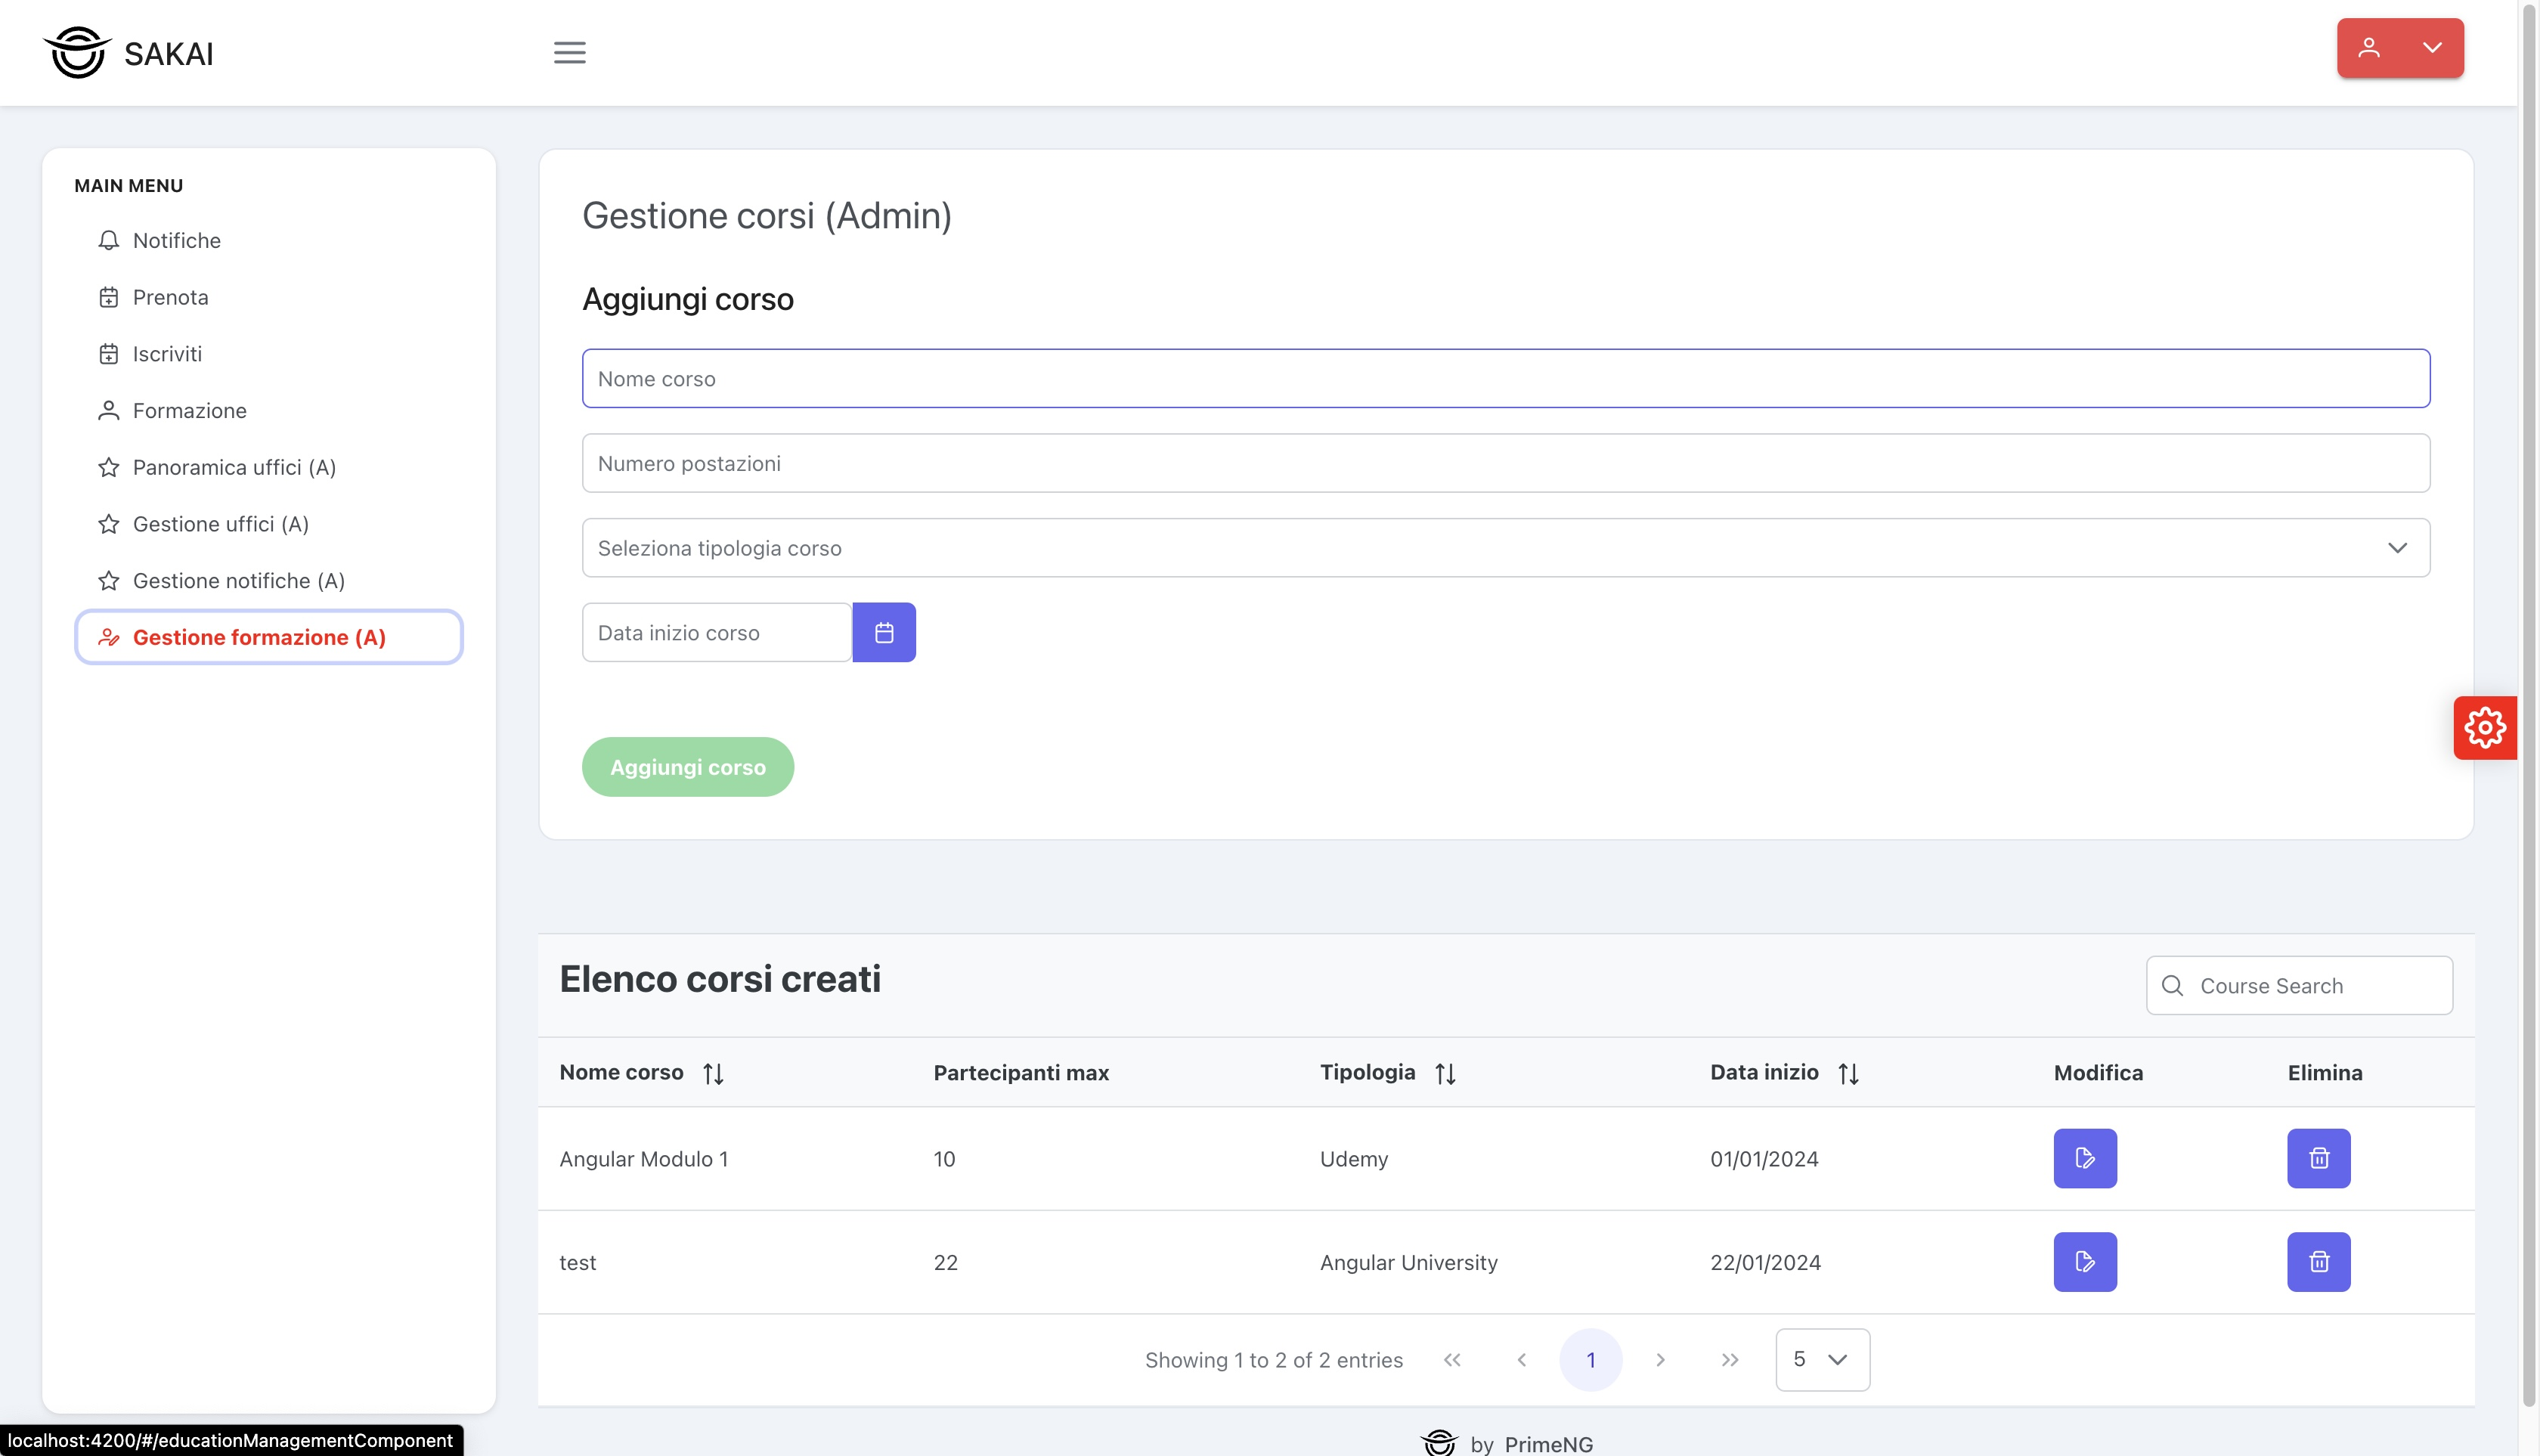
\includegraphics[width=1\textwidth]{Images/portale.jpg}
\caption{\label{fig:portale}Prototipo finale.}
\end{figure}

La figura \ref{fig:portale} mostra una delle pagine del prototipo.

% DB %%%%%%%%%%%%%%%%%%%%%%%%%%%%%%%%%%%%%%%%%%%%%%%%%%%%%%%%%%%%%%%%%%%%%%%%%%%%%%%%%%%%%%%%%%%%%%%%%%%%%%%%
\section{Database}\label{sec:database}
Innanzitutto è stato necessario progettare il database, nello specifico, la creazione di tabelle contenenti le tuple di prova per effettuare il test del prototipo. 
Come da richiesta di Gruppo SIGLA, non è stata realizzata la tabella per la gestione degli utenti, in quanto il progetto di tirocinio si è concentrato principalmente sulle funzionalità dell'amministratore per aggiungere, modificare ed eliminare le attività formative, erogate dall'azienda.

Grazie alle \acrshort{api} di \acrshort{asp.net}, è stato possibile creare la tabella del database direttamente dal codice del back-end. Quindi, è stato utilizzato un \acrfull{orm}, una tecnica che si usa per convertire i dati tra un database relazionale e lo heap\footnote{\glsdesc{heap}} di un linguaggio di programmazione orientato agli oggetti \cite{articleORM}.

Per la tabella dei corsi di formazione, sono stati creati i seguenti campi: 
\begin{itemize}
  \item \texttt{Id del corso} (integer), chiave primaria
  \item \texttt{CoursesName} (string), nome del corso
  \item \texttt{CoursesCapacity} (integer), capacità massima di utenti del corso
  \item \texttt{CoursesType} (string), tipologia del corso
  \item \texttt{CoursesDate} (string), data di inizio del corso
\end{itemize}

Una volta fatto ciò, la tabella che tiene traccia delle versioni del database, `VersionInfo' è stata aggiornata con le nuove migrazioni\footnote{\glsdesc{migrazione}}. Le sue colonne sono:
\begin{itemize}
  \item \texttt{Version} (integer), versione del database
  \item \texttt{AppliedOn} (datetime), data di applicazione della migrazione
  \item \texttt{Description} (text), descrizione della migrazione
\end{itemize}

Per visualizzare e gestire il database, è stato utilizzato DBeaver, un software gratuito e open source per la gestione di database relazionali. La scelta di usare DBeaver è dovuta alla sua semplicità d'uso e al fatto che sia sviluppato dalla comunità open source \cite{dbeaver}.

\begin{figure}[H]
\centering

\includegraphics[width=0.25\textwidth]{Images/dbeaver.png}
\caption{\label{fig:dbeaver}Logo di DBeaver.}
\end{figure}


% back-end %%%%%%%%%%%%%%%%%%%%%%%%%%%%%%%%%%%%%%%%%%%%%%%%%%%%%%%%%%%%%%%%%%%%%%%%%%%%%%%%%%%%%%%%%%%%%%%%%%%%
 
\section{Back-end}\label{sec:back-end}
Questa sezione descrive come ho usato \acrshort{asp.net} per lo sviluppo del back-end del prototipo.

Lo sviluppo principale è stato fatto appoggiandosi all'applicazione web già esistente, sulla quale Gruppo SIGLA ha sviluppato il progetto di tirocinio, che poi offre agli studenti. Quindi, basandomi sull'architettura già esistente, ho creato 5 nuove classi e modificato la classe \texttt{Program.cs}, già esistente, per gestire le funzionalità del prototipo. Queste classi sono:
\begin{itemize}
  \item \texttt{CoursesData.cs}
  \item \texttt{4\_CoursesMigration.cs}
  \item \texttt{CoursesController.cs}
  \item \texttt{CoursesDataGetListExecutor.cs}
  \item \texttt{CoursesDataExecuteExecutor.cs}
\end{itemize}

In particolare, la classe \texttt{CoursesData.cs} è stata creata per definire la tabella `CoursesData' e le sue colonne, tramite la libreria IdentityModel di \acrshort{asp.net}. La classe viene gestita come un'entità grazie all'attributo \texttt{[DbModel]} e le colonne vengono definite come proprietà della classe stessa, coi rispettivi metodi getter\footnote{\glsdesc{getter}} e setter\footnote{\glsdesc{setter}}.
La figura \ref{fig:coursesdata} mostra il codice C\# del file \texttt{CoursesData.cs}.

\begin{figure}[H]
\begin{lstlisting}[linewidth=20cm, captionpos=b]
namespace It.gs.back-end.Model
{
  using System.Text.Json.Serialization;
  using It.gs.Repository;
  using It.gs.Repository.Model;
  public class AddCoursesToDbExecuteInfo : IExecuteInfo {
    public CoursesData[] Courses {get; set; }
  }
  public class DeleteCoursesDataExecuteInfo : IExecuteInfo {
    public CoursesData[] Courses {get; set; }
  }
  public class UpdateCoursesDataExecuteInfo : IExecuteInfo {
    public CoursesData[] Courses {get; set; }
  }
  [DbModel]
  public class CoursesData
  {
      [JsonPropertyName("coursesId")]
      public int CoursesId { get; set; }
    
      [JsonPropertyName("coursesName")]
      public string CoursesName { get; set; }
    
      [JsonPropertyName("coursesCapacity")]
      public int CoursesCapacity { get; set; }
    
      [JsonPropertyName("coursesType")]
      public string CoursesType { get; set; }
    
      [JsonPropertyName("coursesDate")]
      public string CoursesDate { get; set; }
    
      [JsonPropertyName("count")]
      public int? Count { get; set; }
  }
}
\end{lstlisting}
\caption{\label{fig:coursesdata}Codice in C\# del file \texttt{CoursesData.cs}.}
\end{figure}

La classe \texttt{CoursesMigration}, che estende la classe del contesto \texttt{Migration}, si occupa di creare la tabella del database, tramite un \acrshort{orm} \cite{orm} e i metodi appositi della libreria \texttt{FluentMigrator} \cite{fluentmigrator}. In figura \ref{fig:coursesdata} si può vedere il listato del codice relativo alla creazione del database.
\begin{figure}[H]
\begin{lstlisting}
Create.Table($"{nameof(CoursesData)}")
    .WithColumn($"{nameof(CoursesData.CoursesId)}") .AsInt32() .PrimaryKey().Identity()
    .WithColumn($"{nameof(CoursesData.CoursesName)}") .AsBoolean() .NotNullable().WithDefaultValue(false)
    .WithColumn($"{nameof(CoursesData.CoursesCapacity)}") .AsInt16() .NotNullable().WithDefaultValue(10)
    .WithColumn($"{nameof(CoursesData.CoursesType)}") .AsString() .NotNullable()
    .WithColumn($"{nameof(CoursesData.CoursesDate)}") .AsString() .NotNullable();
\end{lstlisting}
\caption{\label{fig:migration}Frammento di codice C\# del file \texttt{4\_CoursesMigration.cs}.}
\end{figure}
Il listato si trova all'interno del metodo \texttt{Up()} della classe \texttt{CoursesMigration}. 

Siccome i metodi \texttt{Up()} e \texttt{Down()} sono ereditati dalla libreria \texttt{FluentMigrator}, è necessario fare un override\footnote{\glsdesc{override}}, riscrivendoli.

Successivamente, ho inizializzato delle tuple di prova all'interno di una lista denominata \texttt{coursesRows} e le ho inserite nella tabella appena creata tramite un ciclo di scorrimento. In figura \ref{fig:insert} si può vedere il listato appena discusso.
\begin{figure}[H]
\begin{lstlisting}
foreach(var course in coursesRows)
    Insert.IntoTable($"{nameof(CoursesData)}").Row(course);
\end{lstlisting}
\caption{\label{fig:insert}Frammento di codice C\# del file \texttt{4\_CoursesMigration.cs}.}
\end{figure}

La classe \texttt{CoursesController}, invece, estende la classe \texttt{ControllerBase}. In particolare, grazie agli attributi \texttt{[HttpPost(" ")]} e \texttt{[ProducesResponseType(400)]}, gestisce le richieste e le risposte \acrshort{http}, smistandole nei metodi responsabili di ognuna delle operazioni (aggiunta, modifica, ricerca o eliminazione). Per esempio, il metodo \texttt{AddCoursesToDb} crea un oggetto contenente le informazioni necessarie all'esecuzione e lo passa come parametro al metodo \texttt{Execute} che eseguirà una delle quattro azioni, a seconda del tipo dell'oggetto in input. In figura \ref{fig:add} si può vedere il listato del metodo appena discusso.
\begin{figure}[H]
\begin{lstlisting}
[HttpPost("addCoursesData")]
[ProducesResponseType(200)]
[ProducesResponseType(400)]
[ProducesResponseType(500)]
public async Task<IActionResult> AddCoursesToDb([FromBody] CoursesData[] Courses) {
    var CoursesInfo = new AddCoursesToDbExecuteInfo {Courses = Courses};
    var result = await this.coursesDataRepo.Execute(CoursesInfo);
    if(result.IsSuccess)
        return Ok();
    else 
        throw result.Error.SourceException;
}
\end{lstlisting}
\caption{\label{fig:add}Metodo \texttt{AddCoursesToDb()} in C\#, del file \texttt{CoursesController.cs}.}
\end{figure}
I metodi relativi alle altre operazioni sono analoghi al codice in figura \ref{fig:add}.


Il metodo \texttt{Execute(...)} è all'interno della classe \texttt{CoursesDataExecuteExecutor}, che si occupa di eseguire l'operazione corretta, a seconda del tipo dell'oggetto (\texttt{info}) che riceve in input. In figura \ref{fig:switch} si può vedere il listato del codice che gestisce lo smistamento delle operazioni.
\begin{figure}[H]
\begin{lstlisting}
public async Task<IExecuteResult> Execute(DatabaseSettings settings, IDbConnection connection, IDbTransaction transaction, IExecuteInfo info)
{
    switch(info) {
        case AddCoursesToDbExecuteInfo i: 
            return await AddCoursesExecute(settings, connection, transaction, i);
        case DeleteCoursesDataExecuteInfo i:
            return await DeleteCoursesDataExecute(settings, connection, transaction, i);
        case UpdateCoursesDataExecuteInfo i:
            return await UpdateCoursesDataExecute(settings, connection, transaction, i);
        default:
            throw new NotSupportedException($"Execute with transaction for type {info.GetType().FullName} not supported");
    }
}
\end{lstlisting}
\caption{\label{fig:switch}Metodo C\# \texttt{Execute()} contenente lo \texttt{switch} relativo alle operazioni.}
\end{figure}

Nel caso in cui \texttt{info} sia di tipo \texttt{AddCoursesToDbExecuteInfo}, verranno eseguiti i metodi \texttt{AddCoursesExecute} e \texttt{Add}, relativi all'aggiunta di una riga alla tabella dei corsi, come si può vedere nei frammenti di codice delle figure \ref{fig:adding} e \ref{fig:get list}.

\begin{figure}[H]
\begin{lstlisting}
private async Task<IExecuteResult> AddCoursesExecute(DatabaseSettings settings, IDbConnection connection, IDbTransaction transaction, AddCoursesToDbExecuteInfo info) {
    foreach(var Course in info.Courses) {
        _ = await Add(settings, connection, transaction, Course);
    }

    return await IExecuteResult.From(\texttt{true});
}
private async Task<CoursesData> Add(DatabaseSettings settings, IDbConnection connection, IDbTransaction transaction, CoursesData item)
{
    Console.WriteLine("item: ",item);
    var sql = $"INSERT INTO CoursesData (CoursesName, CoursesCapacity, CoursesType, CoursesDate) VALUES (@{nameof(CoursesData.CoursesName)}, @{nameof(CoursesData.CoursesCapacity)}, @{nameof(CoursesData.CoursesType)}, @{nameof(CoursesData.CoursesDate)})";

    var r = await connection.ExecuteAsync(sql, item, transaction);
    return item;
}
\end{lstlisting}
\caption{\label{fig:adding}Metodi C\# per l'inserimento dei corsi nel database.}
\end{figure}
In particolare, notiamo che \texttt{AddCoursesToDbExecuteInfo()} chiama \texttt{Add()} e in quest'ultimo vengono effettivamente implementate le query per interrogare il database.

Infine, è degno di nota anche il file \texttt{CoursesDataGetListExecutor.cs}, che si occupa di raccogliere la lista dei corsi di formazione, tramite il metodo \texttt{GetList()}, chiamato dalla classe \texttt{CoursesController} descritta in precedenza.

\begin{figure}[H]
\centerline{(Listato \ref{fig:get list}).}
\begin{lstlisting}
public async Task<IEnumerable<CoursesData>> GetList(DatabaseSettings settings, IDbConnection connection, Maybe<CoreDynamicQueryPart> query)
{
    var (countSql, sql, parameters) = query.EnsureOrderBy(nameof(CoursesData.CoursesId)) .ComposeWithCount<DapperQueryParametersBuilder, DynamicParameters>($"SELECT * $FROM {nameof(CoursesData)}", nameof(CoursesData.CoursesId), settings);
    var result = await connection.QueryAsync<CoursesData>(sql: sql, param: parameters);
    var count = await connection.QuerySingleAsync<int>(sql: countSql, param: parameters);
    return result.Select(x => { x.Count = count; return x; });
}
\end{lstlisting}
\caption{\label{fig:get list}Implementazione del metodo \texttt{GetList.cs} del file C\#  \texttt{CoursesDataGetListExecutor.cs}.}
\end{figure}

Una volta implementato il back-end, per verificare il suo corretto funzionamento, ho utilizzato una \acrshort{api} apposita, Swagger, già discussa nel Capitolo \ref{ch:Contesto}. Nelle figure \ref{fig:swagger courses} e \ref{fig:swagger success} si possono vedere alcuni esempi di utilizzo.

\begin{figure}[H]
\centering
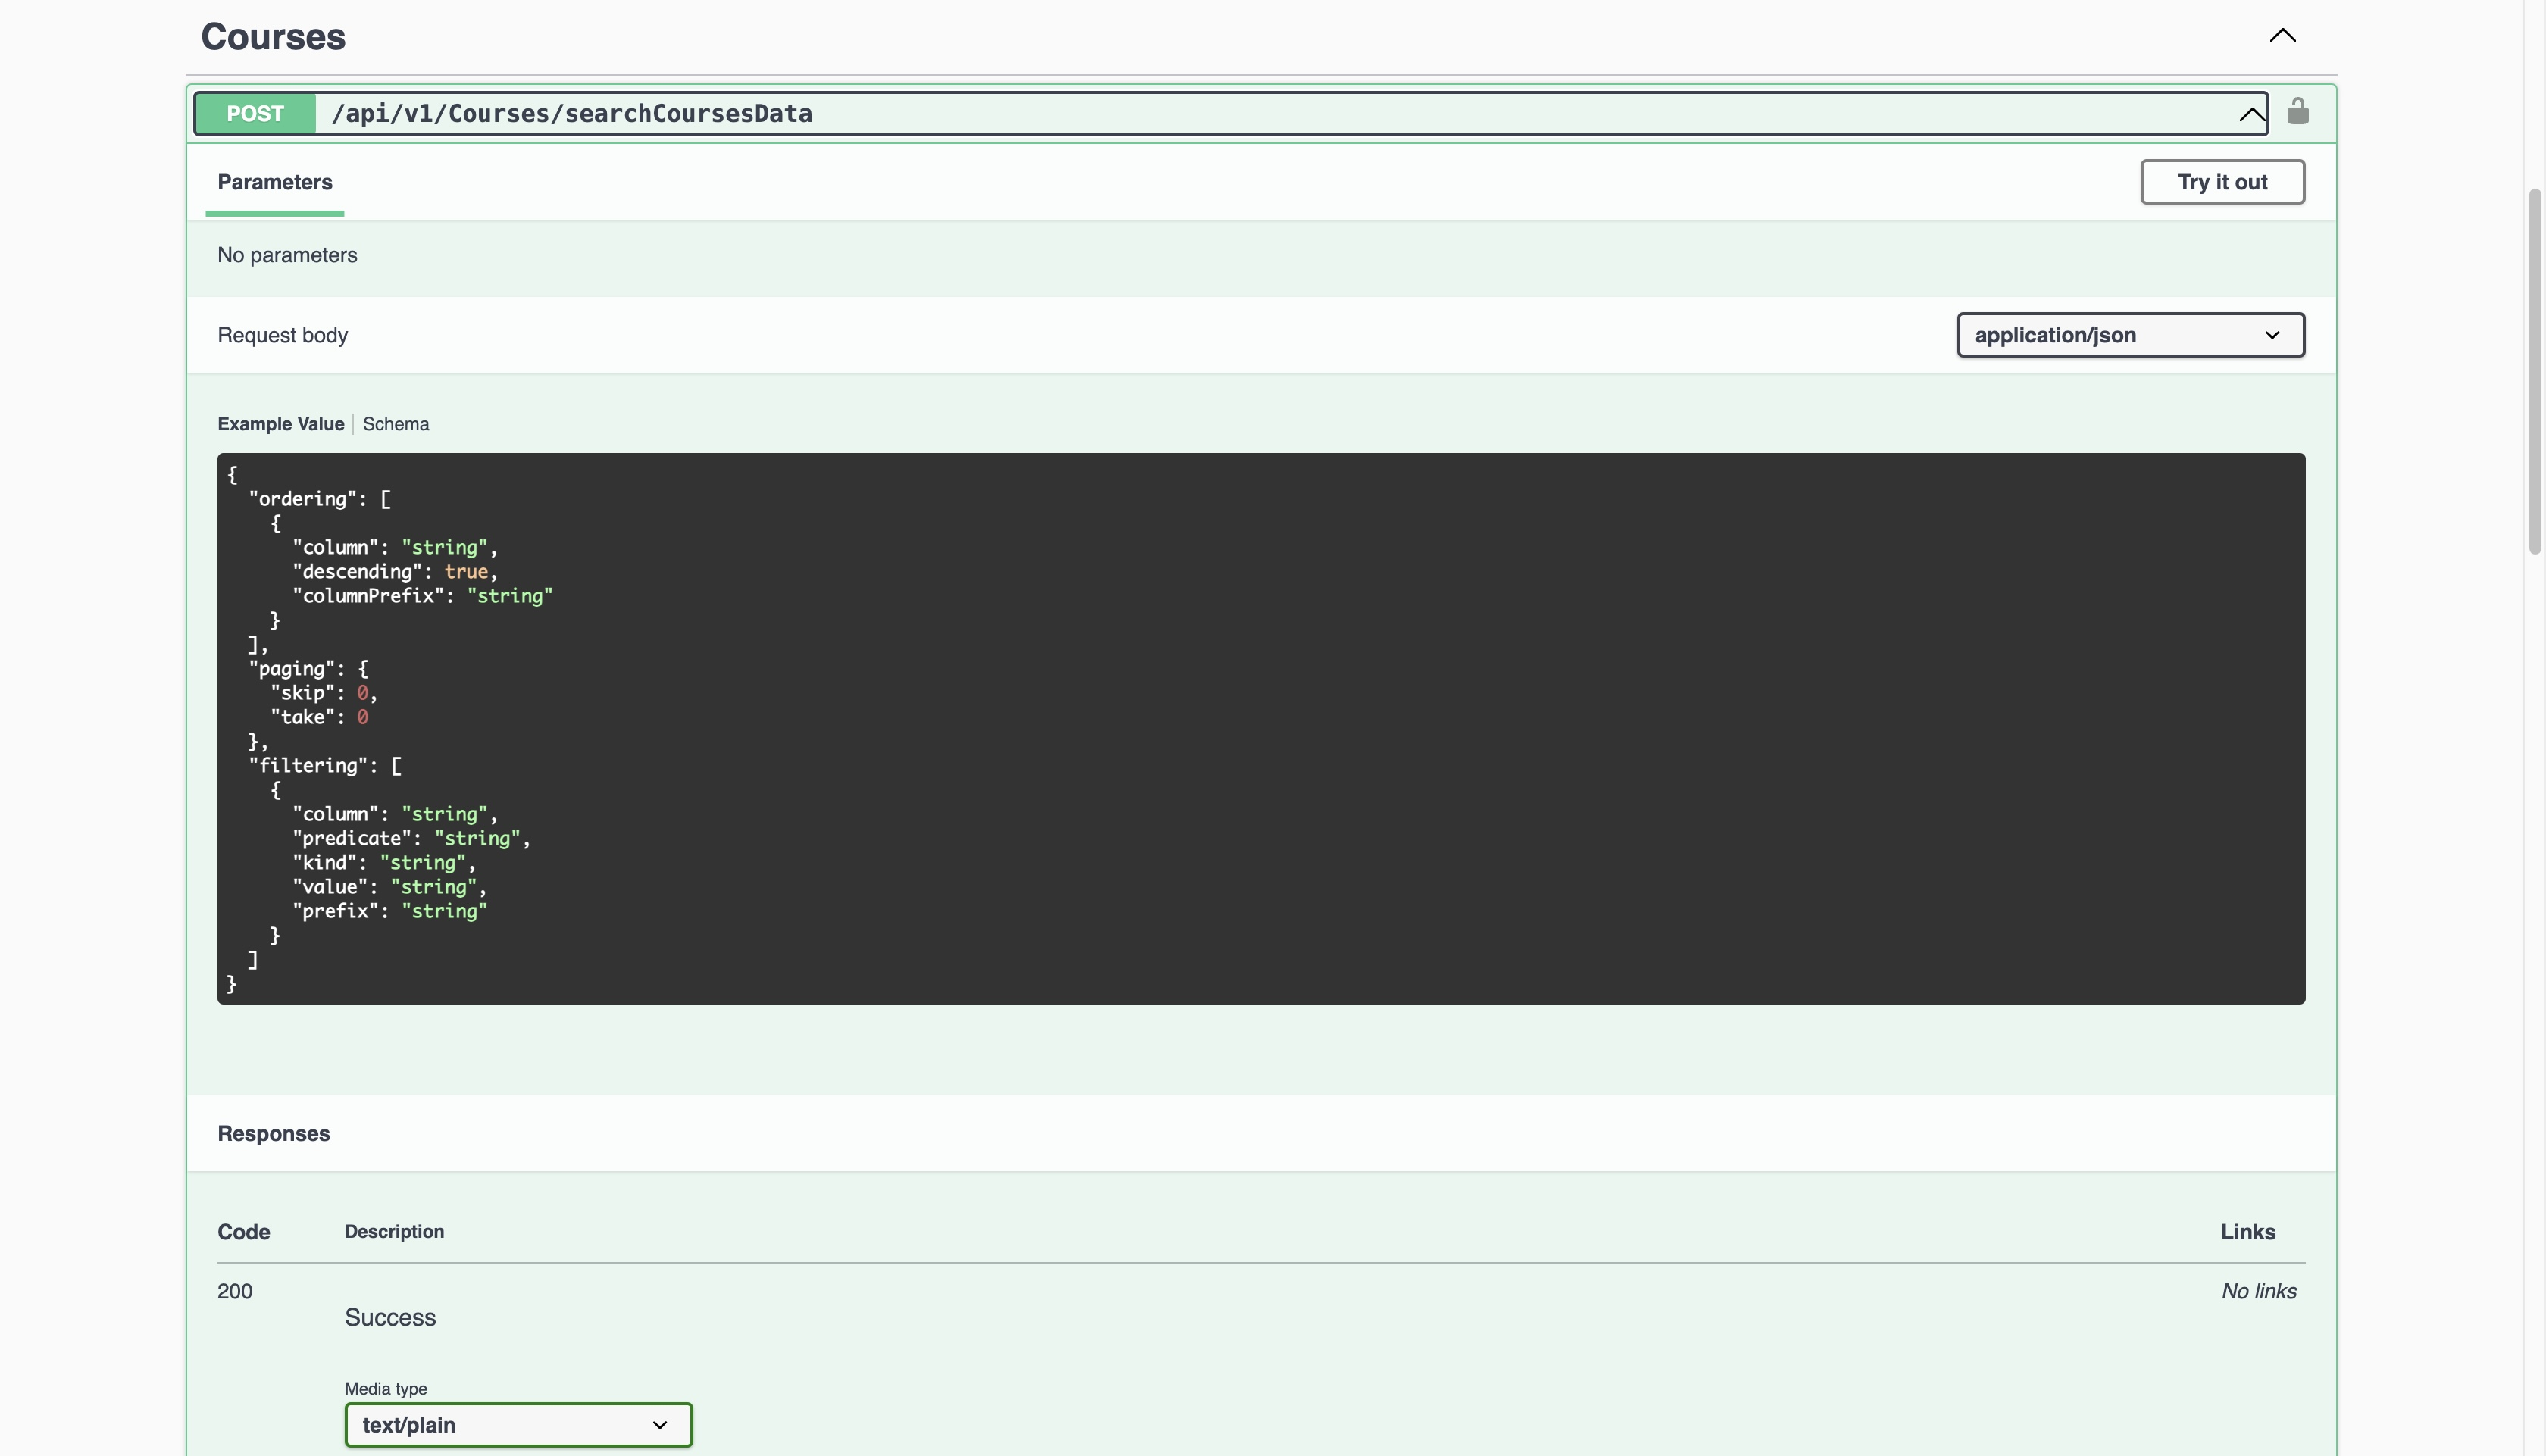
\includegraphics[width=1\textwidth]{Images/swagger courses.jpg}
\caption{\label{fig:swagger courses}Esempio di esecuzione di una \acrshort{api} per \texttt{searchCoursesData}, il corpo della richiesta è in formato \acrshort{json}.}
\end{figure}

\begin{figure}[H]
\centering
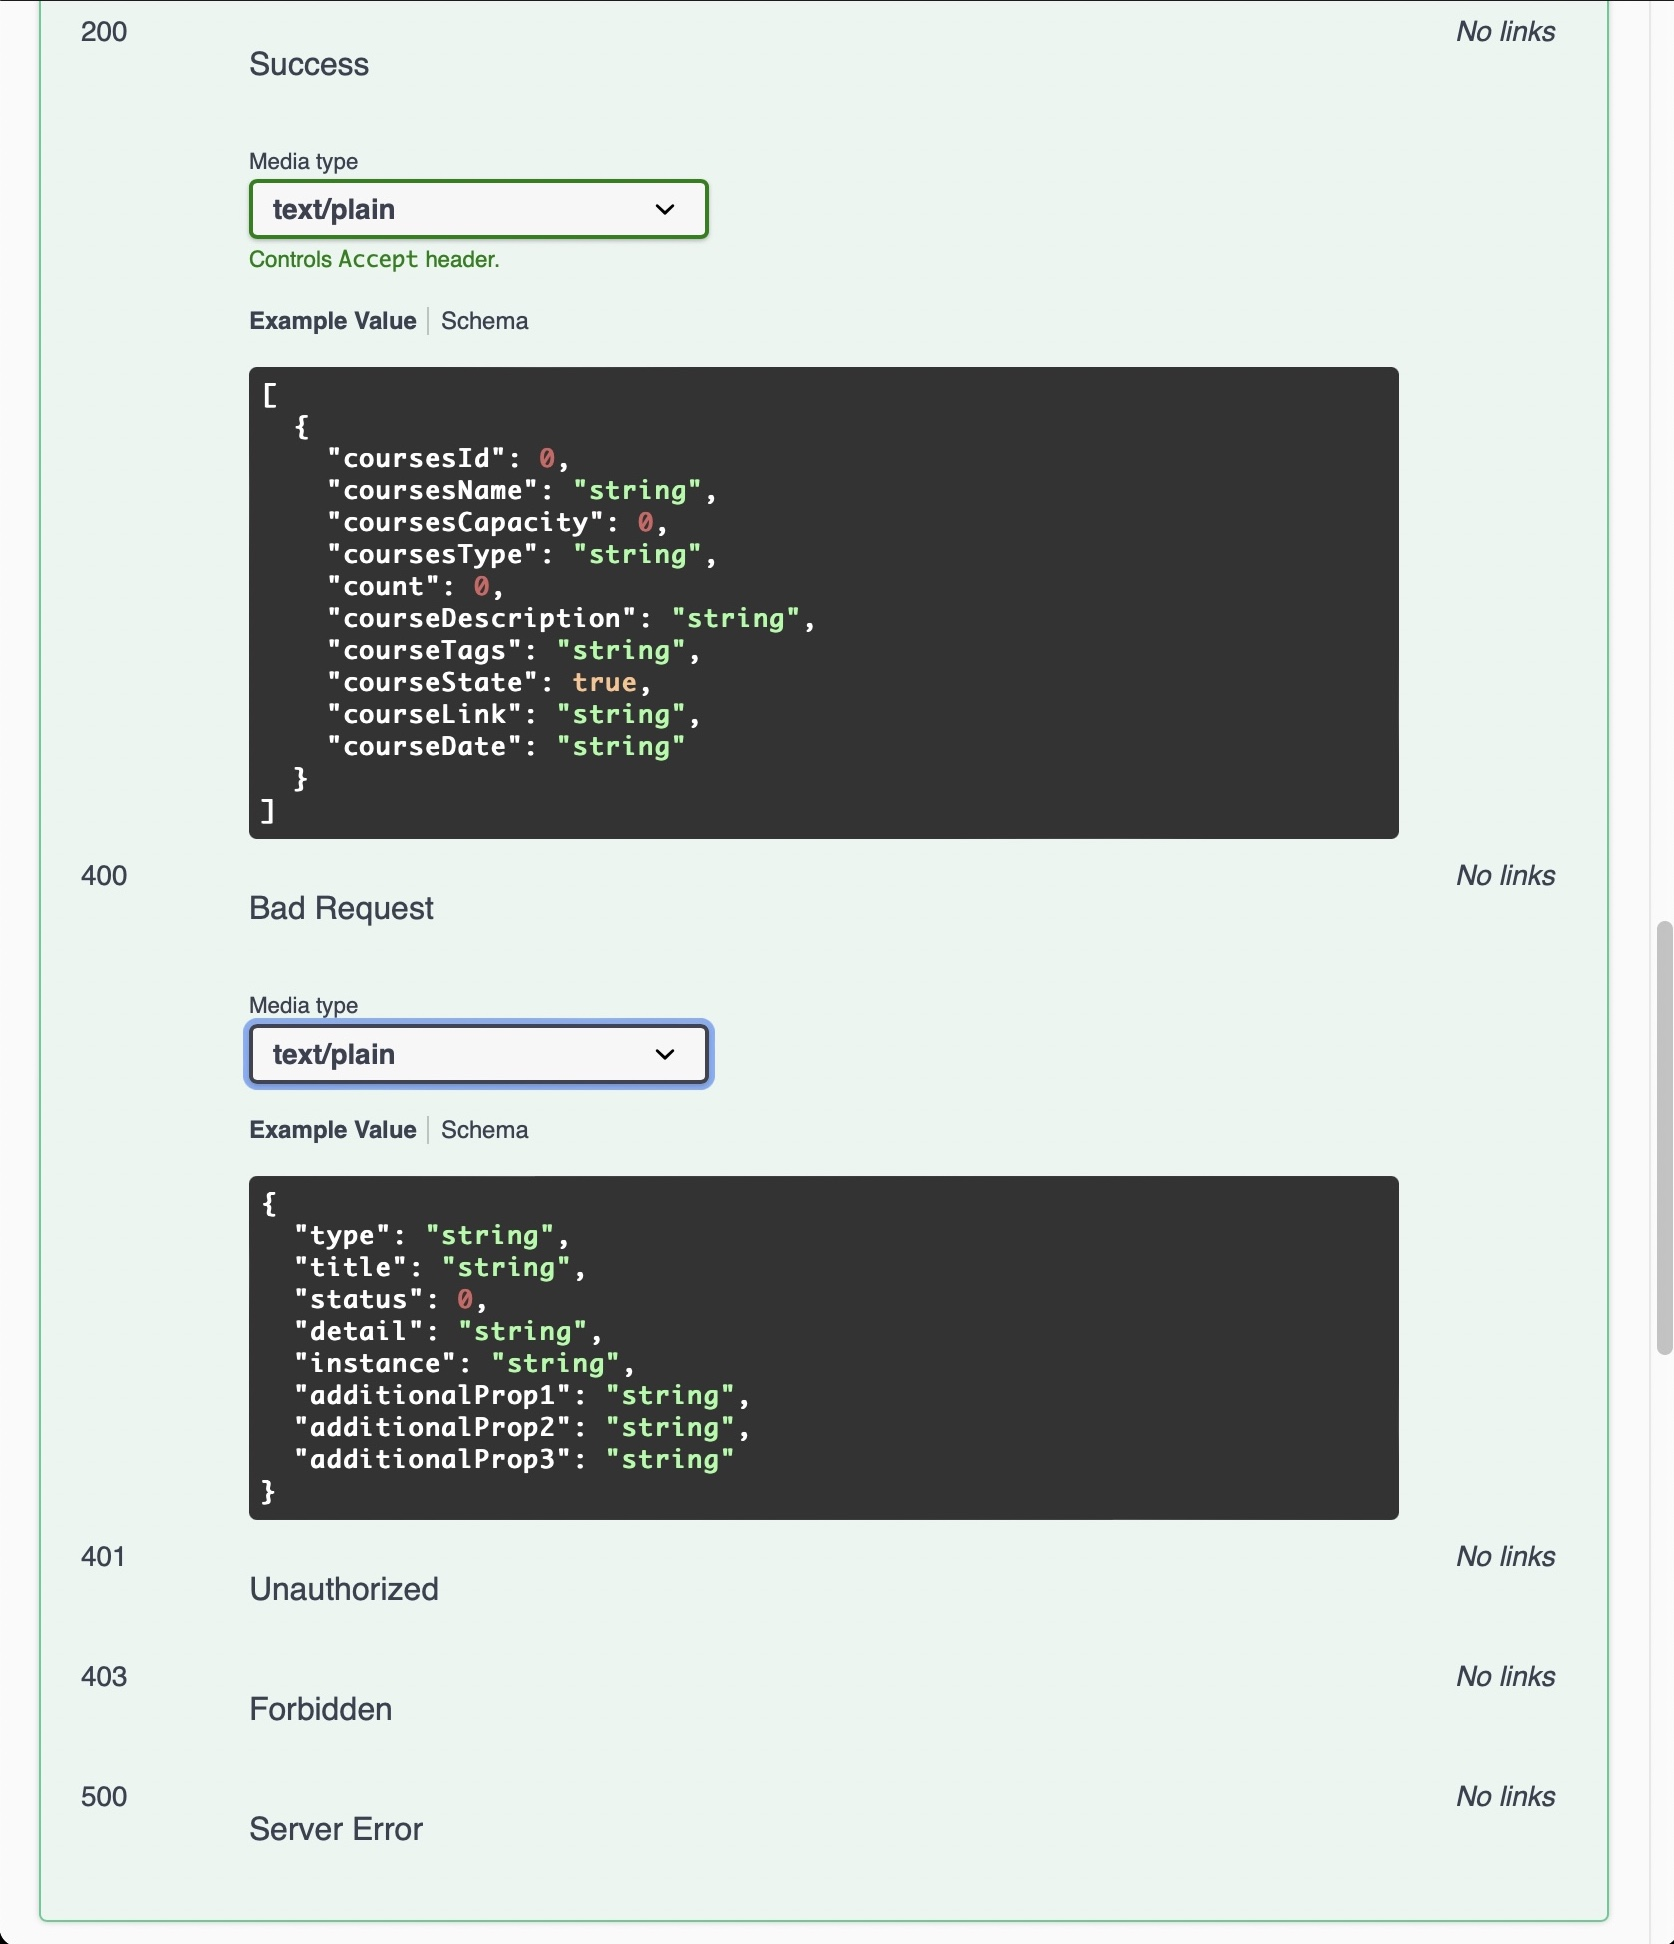
\includegraphics[width=1\textwidth]{Images/swagger success.jpg}
\caption{\label{fig:swagger success}Alcuni esempi di risultati di esecuzione di \acrshort{api} tramite Swagger, in ordine \texttt{200, Successo}, \texttt{400, `Cattiva richiesta'}, \texttt{401, `Non autorizzato'}, \texttt{403, `Vietato'} e \texttt{500, `Errore interno del server'}.}
\end{figure}


% front-end %%%%%%%%%%%%%%%%%%%%%%%%%%%%%%%%%%%%%%%%%%%%%%%%%%%%%%%%%%%%%%%%%%%%%%%%%%%%%%%
\section{Front-end}\label{sec:front-end}
Questa sezione descrive come ho usato \gls{angular} per lo sviluppo del front-end del prototipo.
Innanzitutto è stato necessario installare \acrfull{npm} e \acrfull{nvm}, i gestori di pacchetti rispettivamente per Angular e Node.js. In figura \ref{fig:installing nvm} si può vedere il listato del codice necessario per installarli, da riga di comando:
\begin{figure}[H]
\centering
\begin{lstlisting}[language=bash]
curl -o- https://raw.githubusercontent.com/nvm-sh/nvm/v0.39.0/   install.sh | bash
\end{lstlisting}
\caption{\label{fig:installing nvm}Comando per il terminale per scaricare e installare \acrshort{nvm}.}
\end{figure}
Successivamente, sempre da riga di comando, ho impostato la versione di \acrshort{nvm} necessaria per questo progetto, la numero 16, e poi ho installato le dipendenze necessarie, tramite il comando \texttt{npm install} \cite{nmpInstall}.

A questo punto, ho compilato e avviato il front-end tramite i comandi appositi \texttt{ng build} e \texttt{ng serve} in modo da poter accedere all'interfaccia grafica del prototipo, semplicemente accedendo ad un \acrshort{url} su un qualsiasi browser. Nella figura \ref{fig:ng serve} è mostrato l'output di un esempio di esecuzione del comando \texttt{ng serve} sul terminale.
\begin{figure}{}
\centering
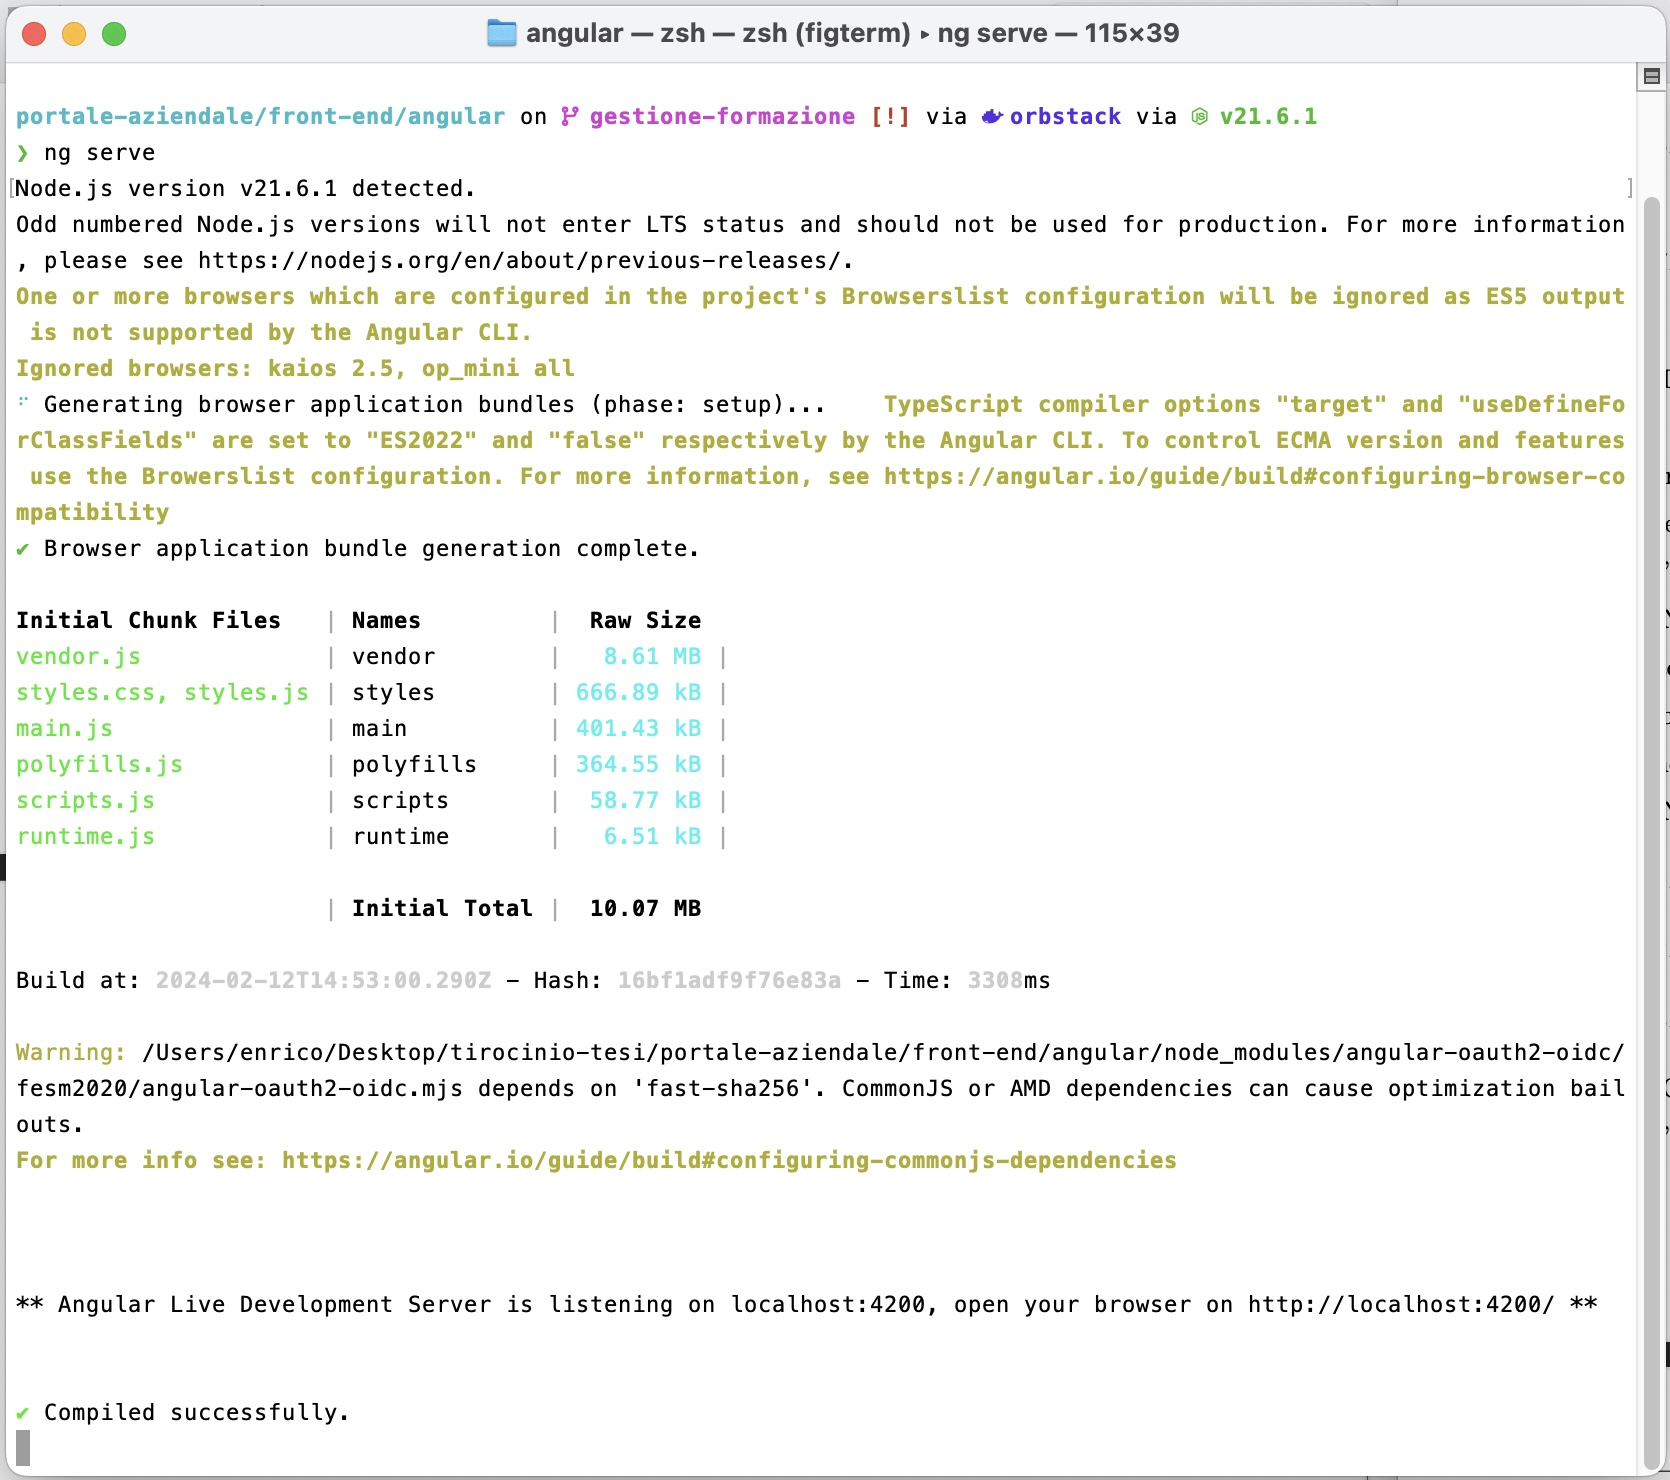
\includegraphics[width=.8\textwidth]{Images/ng serve.jpg}
\caption{\label{fig:ng serve}Screenshot di un terminale dopo aver eseguito \texttt{ng serve}.}
\end{figure}

Per la parte di sviluppo in \gls{angular}, ho utilizzato la sua \acrshort{cli}, che mi ha permesso di creare nuovi componenti, direttamente da terminale, con un solo comando. Per installarla è bastato eseguire \texttt{npm install -g @angular/cli} da riga di comando.
Se un nuovo componente viene creato senza errori, verrà creata una nuova cartella, chiamata con il nome del componente, all'interno del percorso \texttt{src/app/components}.
La cartella contiene fin dall'inizio tutti i file necessari per far funzionare il nuovo componente, come si può vedere in figura \ref{fig:education}.
\begin{figure}[H]
\centering
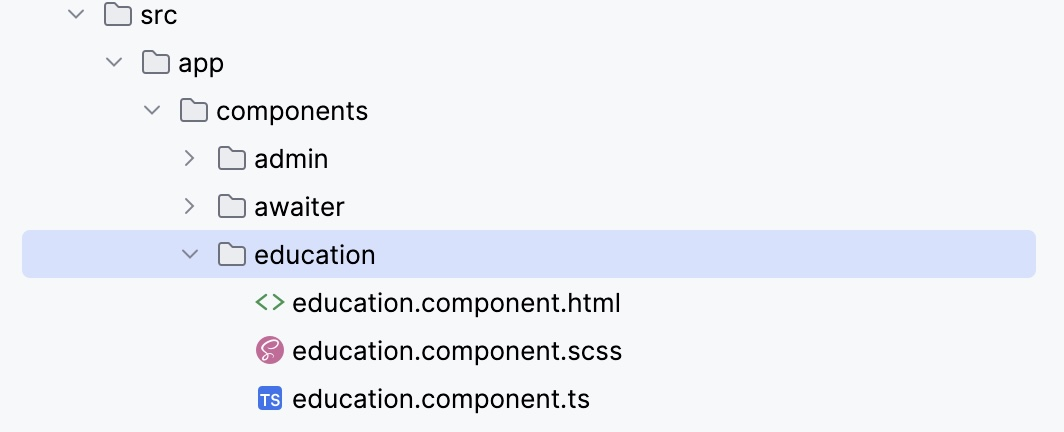
\includegraphics[width=1\textwidth]{Images/education.jpg}
\caption{\label{fig:education}Struttura della cartella del componente \texttt{education}, creata tramite la \acrshort{cli} di Angular.}
\end{figure}

Una volti creati i componenti, ho sviluppato il file \texttt{app-routing.module.ts}, che contiene la route guard di \gls{angular}. 
\begin{figure}[H]
\centering
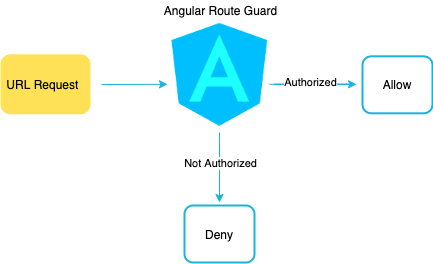
\includegraphics[width=.8\textwidth]{Images/routeguard.png}
\caption{\label{fig:routeguard}Schema di instradamento di \gls{angular}.}
\end{figure}
Una \texttt{route guard} in Angular è un meccanismo utilizzato per proteggere l'instradamento dell’applicazione e limitare l’accesso alle pagine in base alle autorizzazioni dell’utente. Le guardie consentono di gestire la navigazione dell’utente in modo sicuro, garantendo l’accesso alle pagine riservate solo agli utenti autorizzati (figura \ref{fig:routeguard}).
Una \texttt{route guard} è una classe \acrlong{ts} che implementa l’interfaccia \texttt{canActivate}, i cui metodi vengono eseguiti quando un utente tenta di accedere a una determinata rotta dell’applicazione.
Il metodo \texttt{canActivate}, ad esempio, viene eseguito quando un utente tenta di accedere a una route specifica. La \texttt{route guard} può quindi verificare se l’utente ha l’autorizzazione per accedere alla route e restituire un valore booleano che indica se l’accesso deve essere consentito o meno. Se la \texttt{route guard} restituisce \texttt{true}, l’utente può accedere, se invece restituisce \texttt{false}, l’utente viene reindirizzato a una pagina di errore o alla pagina di login. In figura \ref{fig:route guard} si può vedere il listato di un frammento di codice di una \texttt{route guard} sviluppata per questo progetto di tirocinio.
\begin{figure}[H]
\centering
\begin{lstlisting}[language=TypeScript]
export class AdminUserGuard implements canActivate {
    constructor(private oauthService: CustomOAuthService) {}

    async canActivate(
        route: ActivatedRouteSnapshot,
        state: RouterStateSnapshot
    ): Promise<boolean | UrlTree> {
        const isAdminUser = await this.oauthService.isAdminUser();
        if (!isAdminUser)
            console.error("You should be 'admin-user' to activate this route!");
        return isAdminUser;
    }
}
\end{lstlisting}
\caption{\label{fig:route guard}Metodo \texttt{canActivate} del file \texttt{admin-user.guard.ts}.}
\end{figure}
Una volta sviluppato il codice in figura \ref{fig:route guard} è stato necessario implementare il codice relativo al file \texttt{app-routing.module.ts} e l'instradamento dell'utente è completato. Il risultato è mostrato nelle seguenti figure.

\begin{figure}[!htb]
    \centering
    \begin{minipage}{.5\textwidth}
        \centering
        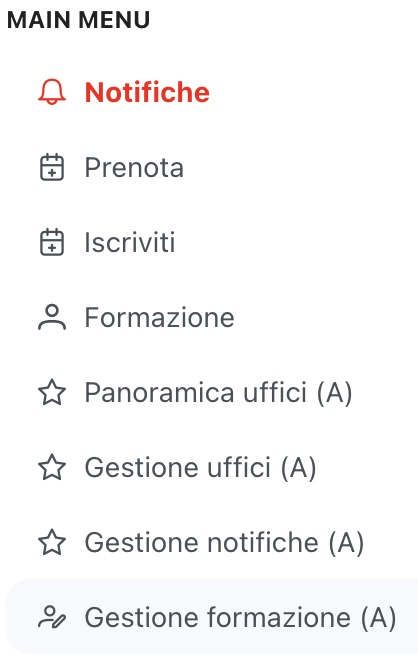
\includegraphics[width=.6\textwidth]{Images/admin.jpg}
        \centering
        \caption{\label{fig:admin}Vista dell'admin.}
    \end{minipage}%
    \begin{minipage}{0.5\textwidth}
        \centering
        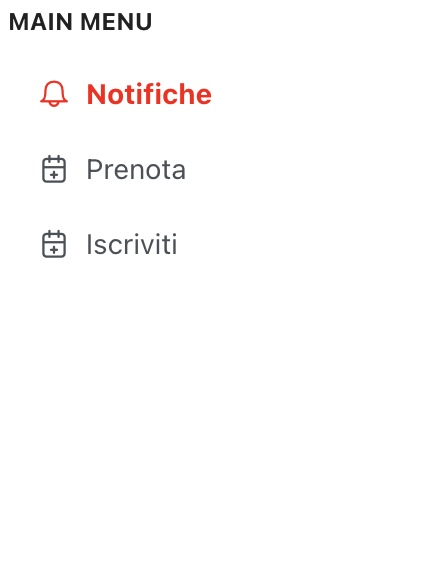
\includegraphics[width=.5\textwidth]{Images/base.jpg}
        \caption{\label{fig:base}Vista dell'utente base.}
    \end{minipage}
\end{figure}

Il codice di ogni componente è diviso nei tre file seguenti:
\begin{itemize}
  \item \texttt{`name'.component.html}, che si occupa di gestire la parte \acrshort{html} del componente, è quindi il template dello stesso;
  \item \texttt{`name'.component.ts}, che si occupa di gestire la parte TypeScript del componente;
  \item \texttt{`name'.component.css}, che in questo caso è vuoto, siccome il \acrshort{css} di ogni componente è stato gestito tramite il file \texttt{styles.css}.
\end{itemize}

In particolare, il file \acrshort{html} contiene lo `scheletro' del componente da visualizzare e alcuni tag speciali di \gls{angular} come, ad esempio, \texttt{ng-template pTemplate} nel listato \ref{fig:ptemplate}, che si occupa di uniformare i dati del back-end con le relative caselle di una tabella \acrshort{html}.

\begin{figure}[H]
\centering
\begin{lstlisting}[language=HTML]
 <ng-template pTemplate="body" let-coursesData>
    <tr class="p-selectable-row" [pRowToggler]="coursesData.coursesId">
        <td>
            <button type="button" pButton pRipple
                class="p-button-text p-button-rounded p-button-plain"
                [icon]="isRowExpanded(coursesData.coursesId) ? 'pi pi-chevron-down' : 'pi pi-chevron-right'"
                (click)="toggleRow(coursesData.coursesId)">
            </button>
        </td>
        <td>
            <span class="p-column-title">Nome corso</span>
            {{coursesData.coursesName}}
        </td>
    </tr>
</ng-template>
\end{lstlisting}
\caption{\label{fig:ptemplate}Frammento di codice \acrshort{html} del file \texttt{education.component.html}.}
\end{figure}

Per la parte \acrlong{ts} del componente, invece, è stato necessario considerare sia il livello di presentazione, che il livello di database, in modo da gestire e presentare le informazioni correttamente.
\begin{figure}[H]
\centering
\begin{lstlisting}[language=TypeScript]
addEducation(){
this.coursesData$.subscribe((data) => {
    if(data) {
        data.forEach((course) => {
            console.log(course);
    });}
});
\end{lstlisting}
\caption{\label{fig:education.ts}Metodo \texttt{addEducation()} del file \texttt{education.component.ts}.}
\end{figure}
Come mostrato in figura \ref{fig:education.ts}, il codice si occupa di aggiungere le informazioni trovate dal database (salvate in \texttt{coursesData\$()}) al front-end, in modo da essere visualizzate dall'utente.

\begin{figure}[H]
\centering
\begin{lstlisting}[language=CSS]
$gutter: 1rem; //for primeflex grid system
@import "assets/layout.scss";
@import "../node_modules/primeng/resources/primeng.min.css";
@import "../node_modules/primeflex/primeflex.scss";
@import "../node_modules/primeicons/primeicons.css";
@import "assets/overrides/styles/theme.scss";  
\end{lstlisting}
\caption{\label{fig:styles}\acrshort{css} del file \texttt{styles.css}, per gestire il \acrshort{css} di tutti i componenti.}
\end{figure}

La figura \ref{fig:styles} mostra lo stile dei componenti. Ho deciso di usare un tema predefinito di \acrshort{primeng}, importato nel file \texttt{styles.css}, come si può vedere nella figura. Nonostante la leggera perdita di personalizzazione, la scelta di utilizzare un tema predefinito mi ha permesso di ridurre i tempi di sviluppo, in quanto è stato necessario solamente importare un tema già pronto e non scrivere codice \acrshort{css} partendo da zero, cosa spesso complicata.

Altri file degni di nota sono:
\begin{itemize}
  \item \texttt{courses.actions.ts}: contiene tutti gli \texttt{export} delle azioni relative ai corsi di formazione;
  \item \texttt{courses.effects.ts}: si occupa principalmente di mappare le informazioni in entrata o in uscita dal componente;
  \item \texttt{courses.reducer.ts}: contiene alcuni metodi ausiliari per il corretto funzionamento della logica di business, in particolare per filtrare o manipolare le informazioni dal o verso il back-end;
  \item \texttt{courses.state.ts}: contiene la struttura di base dello stato dei corsi di formazione;
  \item \texttt{courses.selectors.ts}: che contiene gli \texttt{export} necessari per il funzionamento di ogni metodo filtro o di stato dei corsi di formazione.
\end{itemize}

Inoltre, dopo aver completato i file citati sopra, ho aggiunto un componente \gls{angular} per visualizzare un calendario visibile a larghezza intera, come si può vedere nella figura \ref{fig:fullcalendar} della pagina dell'applicazione web. Così facendo, l'utente può visualizzare i corsi di formazione esistenti e scegliere il corso di formazione più adatto alle proprie esigenze.
\begin{figure}[H]
\centering
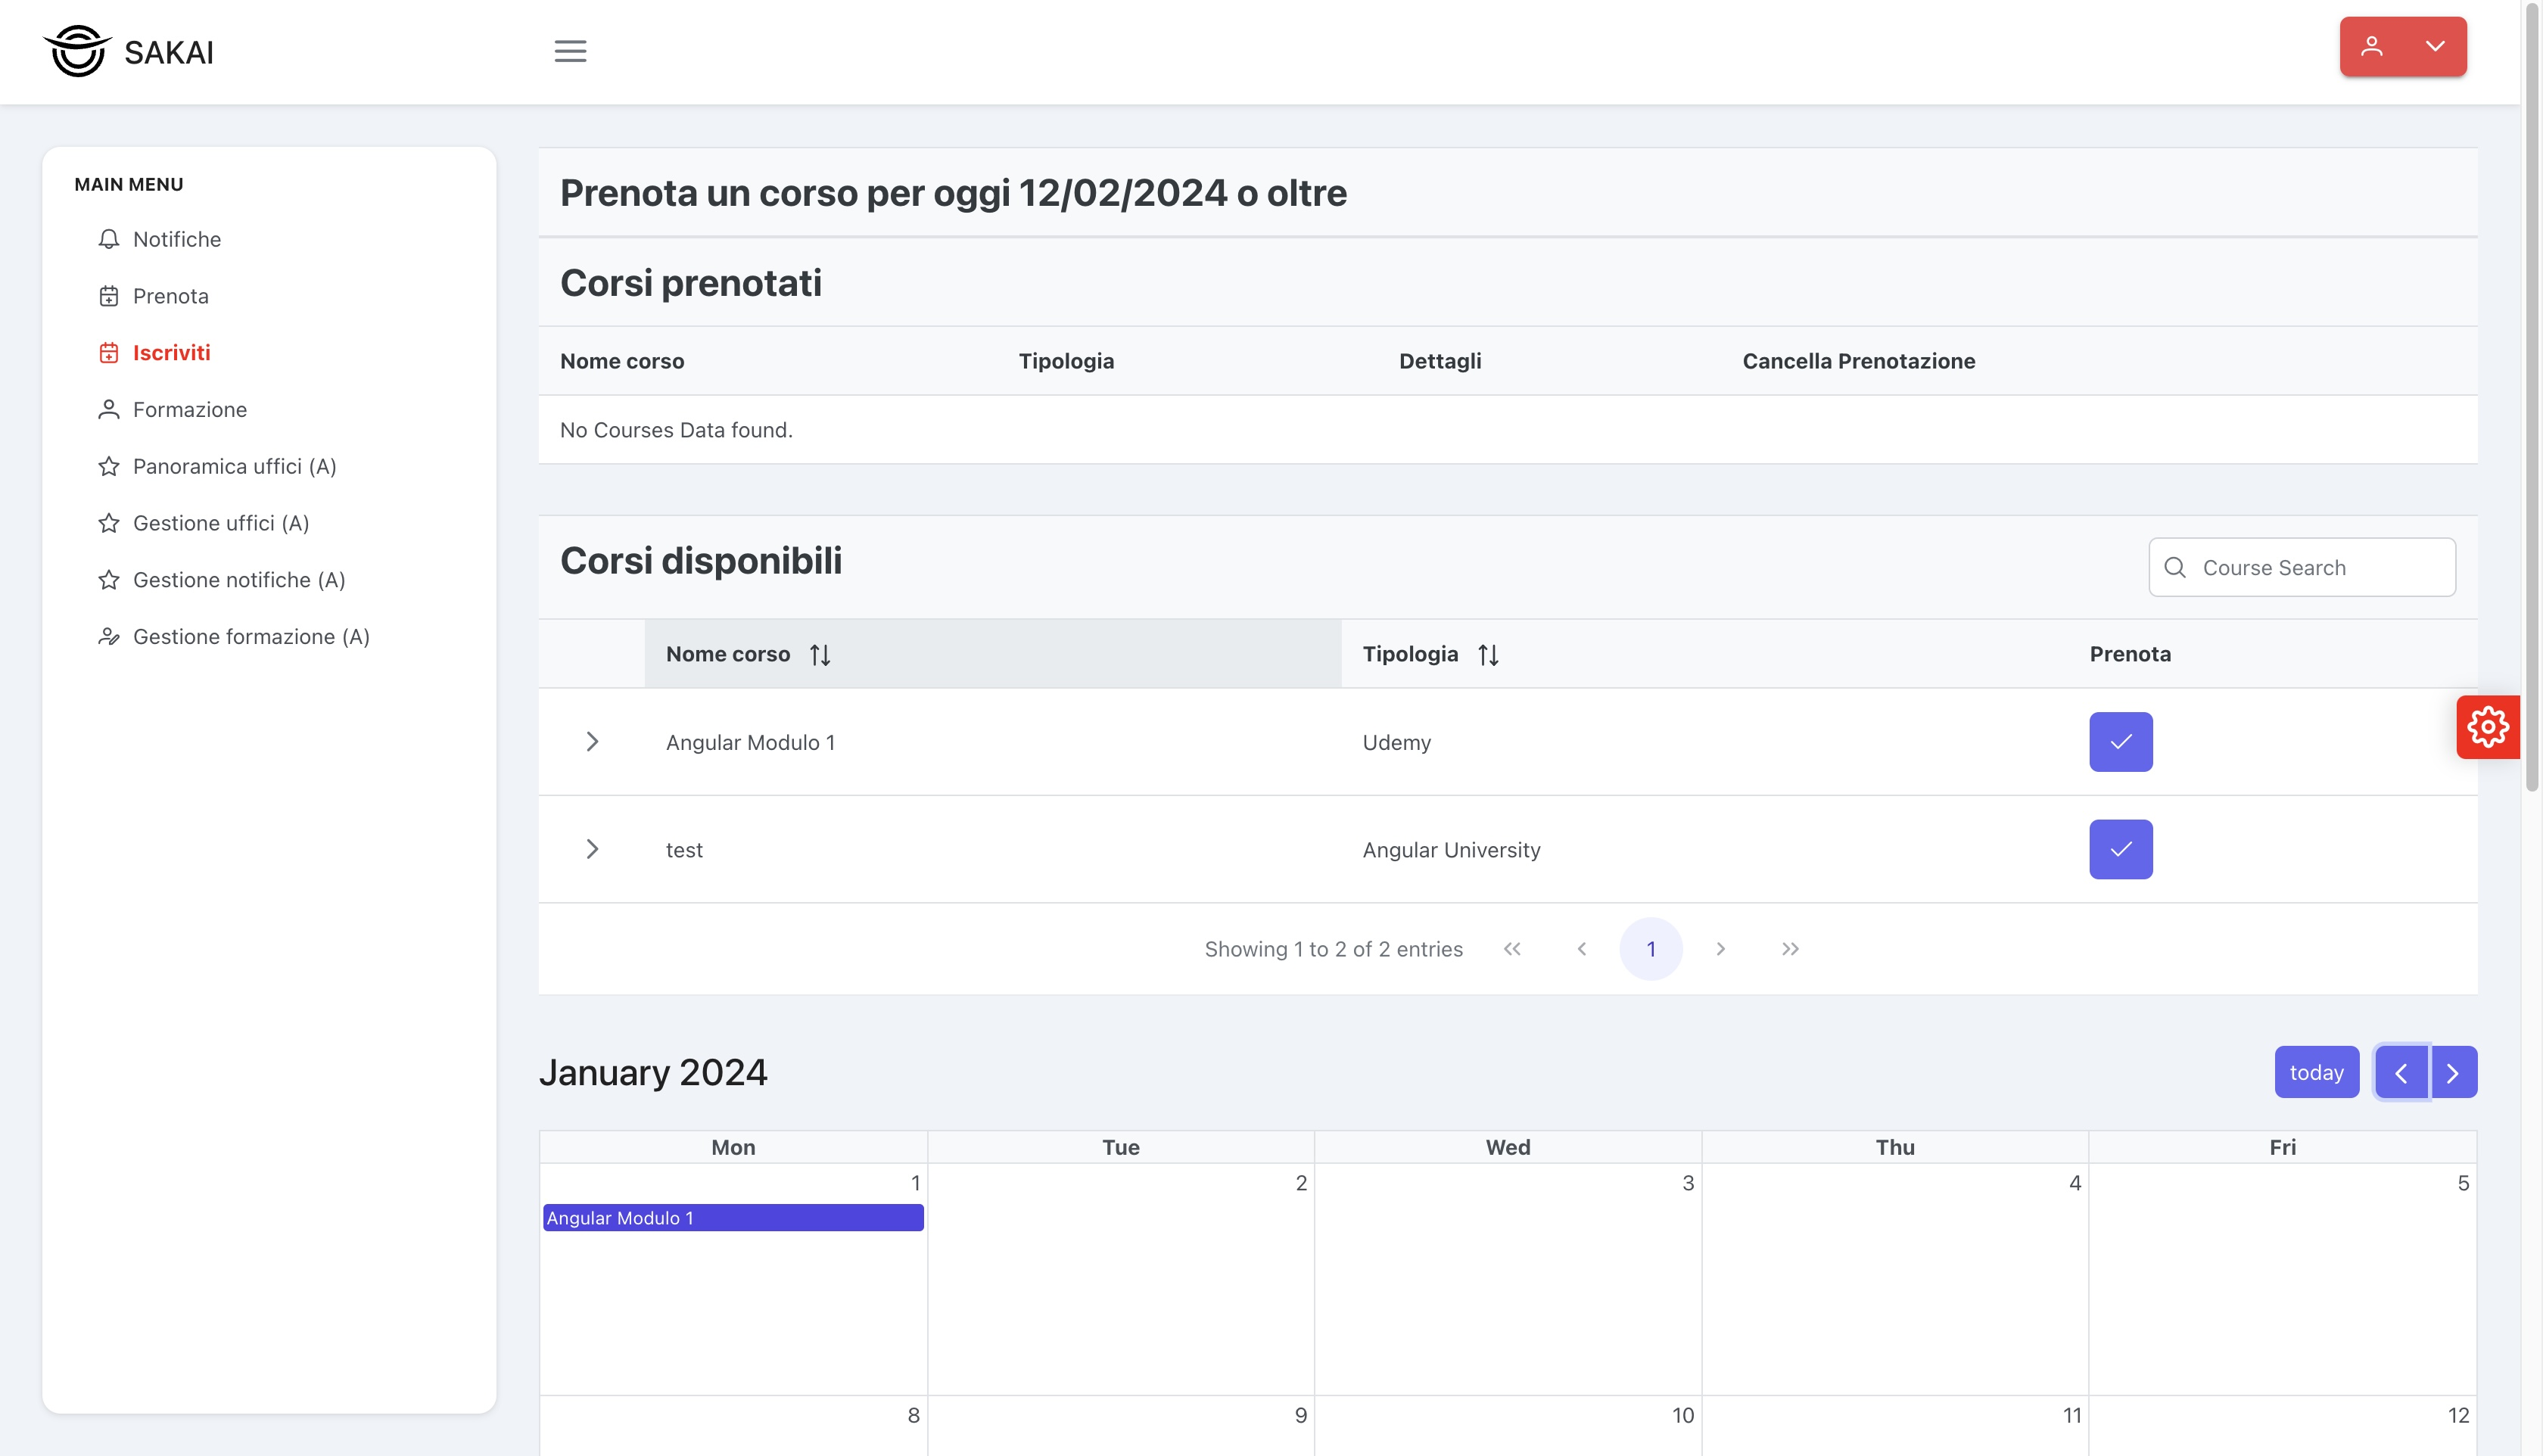
\includegraphics[width=1\textwidth]{Images/calendar cut.jpg}
\caption{\label{fig:calendar}Vista iniziale di una pagina web del prototipo, con il componente \texttt{fullcalendar}.}
\end{figure}

Dopo averlo installato, sempre tramite la \acrshort{cli} di \gls{angular} e aver configurato i file \texttt{app.module.ts} e \texttt{app.component.ts}, il calendario può funzionare correttamente \cite{fullcalendar}, come si può vedere in figura \ref{fig:fullcalendar}, semplicemente aggiungendo il tag \acrshort{html} apposito, mostrato nella figura \ref{fig:fullcalendar.html}:
\begin{figure}[H]
\centering
\begin{lstlisting}[language=HTML]
<full-calendar [options]="calendarOptions"></full-calendar>
\end{lstlisting}
\caption{\label{fig:fullcalendar.html}Tag \acrshort{html} del file \texttt{education.component.html}.}
\end{figure}

\begin{figure}[H]
\centering
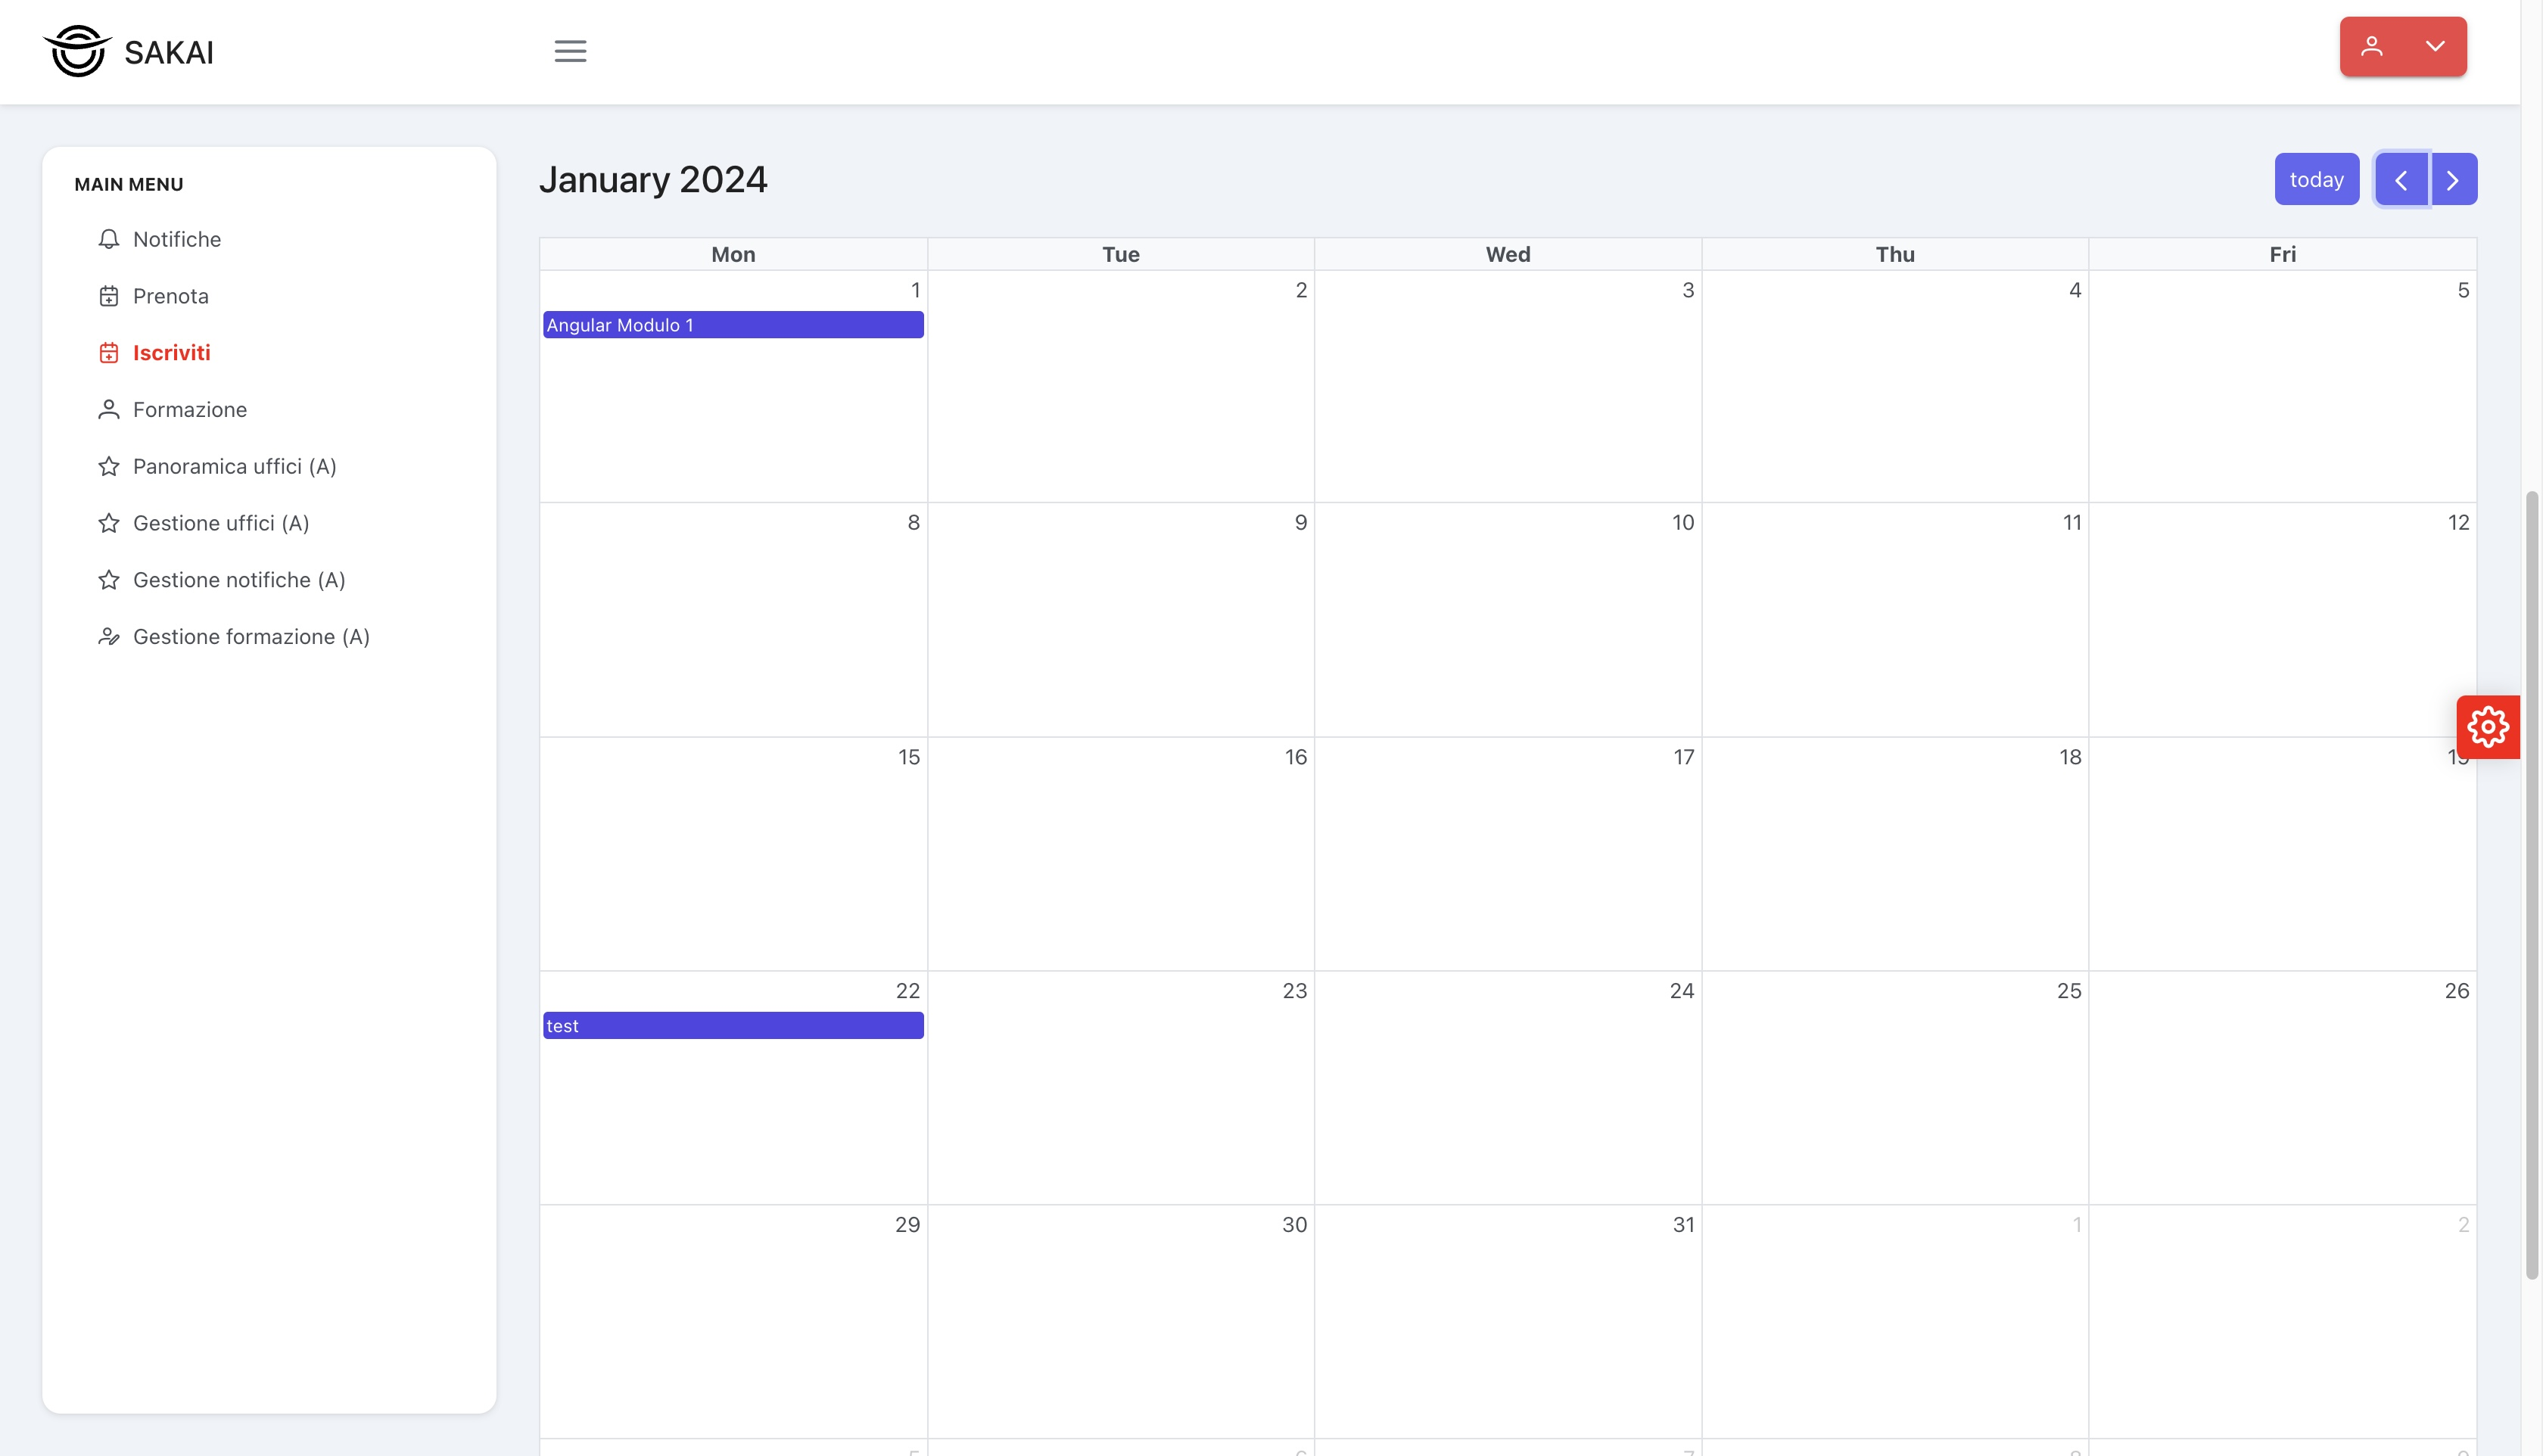
\includegraphics[width=1\textwidth]{Images/fullcalendar.jpg}
\caption{\label{fig:fullcalendar}Componente \texttt{fullcalendar}.}
\end{figure}

In figura \ref{fig:fullcalendar.ts} si può vedere il listato del codice \acrlong{ts}, per gestire la logica di business del componente \texttt{fullcalendarComponent}.

\begin{figure}[H]
\centering
\begin{lstlisting}[language=TypeScript]
ngOnInit(): void {
  this.coursesData$ = this.store.select(selectCoursesData).pipe(startWith( this.route .snapshot.data.CoursesData));
  this.coursesData$.pipe(
      filter(data => !!data)
  ).subscribe((data) => {
      this.totalRecords$ = this.coursesData$.pipe(map((x) => (x ? (x[0] ? x[0].count : 0) : 0)));
      let tmp = [];
      data.forEach((course) => {
          let day:string = course.coursesDate[0] + course.coursesDate[1];
          let month:string = course.coursesDate[3] + course.coursesDate[4];
          let year:string = course.coursesDate[6] + course.coursesDate[7] + course.coursesDate[8] + course.coursesDate[9];
          tmp.push({ title: course.coursesName, date: year + '-' + month + '-' + day }); // yyy-mm-dd
          console.log(tmp);
      });
      this.calendarOptions = {
          ...this.calendarOptions,
          events: tmp
      };
  })
}
\end{lstlisting}
\caption{\label{fig:fullcalendar.ts}\acrlong{ts} del file \texttt{education.component.ts}, necessario per il funzionamento della logica di business del calendario.}
\end{figure}

Lo sviluppo degli altri metodi e componenti è coerente agli esempi mostrati in precedenza e non verrà descritto in questo documento.
Infine, nella fase finale del tirocinio, ho aggiunto un componente per la gestione delle iscrizioni da parte degli utenti base. 
Anche in questo caso il codice è analogo ai file discussi in precedenza e non verrà descritto.


\subsection{PrimeNG}\label{subsec:primeng}
% Una veloce digressione su PrimeNG e su come l'ho usato e perchè \dots
Grazie a \acrshort{primeng}, ho potuto implementare un'interfaccia grafica funzionale e minimale.
Innanzitutto, è stato necessario installare i giusti pacchetti e le giuste dipendenze. Successivamente, la scelta dei componenti utilizzati e descritti in precedenza, è stata fatta in base alle esigenze del progetto e alle funzionalità offerte da \acrshort{primeng}.
In particolare, i componenti usati sono:
\begin{itemize}
  \item \texttt{p-table}, per la visualizzazione dei corsi di formazione;
  \item \texttt{p-sortableColumn} e \texttt{p-sortIcon}, per l'ordinamento dei dati della tabella;
  \item \texttt{p-inputText}, \texttt{p-dropdown}, \texttt{p-calendar}, per la gestione dei campi di input e delle date (figura \ref{fig:dropdown});
  \item \texttt{p-button}, per la gestione dei pulsanti di modifica e cancellazione;
  \item \texttt{p-fullCalendar}, per la visualizzazione dei corsi di formazione esistenti in un calendario;
  \item \texttt{ngtemplate}, per la gestione dei template personalizzati.
\end{itemize}
\begin{figure}[H]
\centering

\includegraphics[width=1\textwidth]{Images/dropdown.jpg}
\caption{\label{fig:dropdown}Menù a tendina per la selezione della tipologia di un corso.}
\end{figure}


\subsection{Servizi Angular}\label{subsec:servizi-angular}
% Una veloce digressione sui servizi Angular e come sono stati usati \dots
I servizi \gls{angular} sono tra le funzionalità più potenti e flessibili del \gls{framework}, in quanto permettono di creare e gestire la logica di business in modo efficiente e modulare \cite{angserv}. Durante questo tirocinio, sono stati usati al fine di gestire la comunicazione tra il livello di presentazione e il livello della logica di business. Inoltre, sono stati scelti per la loro capacità di essere iniettati in qualsiasi componente.
Di seguito (figura \ref{fig:angular service} e \ref{fig:angular service 2}), si possono vedere due esempi di come è stato usato un servizio \gls{angular} per la gestione dei corsi di formazione:
\begin{figure}[H]
\centering
\begin{lstlisting}[language=TypeScript]
  @Injectable({ providedIn: "root" })
\end{lstlisting}
\caption{\label{fig:angular service}\acrlong{ts} del file \texttt{course.resolver.ts}, contenente l'implementazione di un servizio \gls{angular}.}
\end{figure}

\begin{figure}[H]
\centering
\begin{lstlisting}[language=TypeScript]
  @Injectable({ providedIn: "any" })
\end{lstlisting}
\caption{\label{fig:angular service 2}\acrlong{ts} del file \texttt{admin-user-guard.ts}, contenente l'implementazione di un servizio \gls{angular}.}
\end{figure}

% `

\chapter{Conclusioni}\label{ch:conclusioni}
Concludendo, l'utilizzo a 360° degli strumenti e delle tecnologie discusse in questo documento è stato essenziale per la realizzazione di questo progetto di prova finale. 

Dopo aver studiato e approfondito l'architettura del modello three-tier e la documentazione necessaria per lo sviluppo, posso ritenermi soddisfatto dell'esperienza svolta.
Il tirocinio ha fornito un'ottima occasione per approfondire le mie capacità in alcuni linguaggi e impararne altri.
L'applicazione web finale è risultata moderna e intuitiva, al passo coi \gls{framework} odierni. 

Il portale di sviluppo, fornito da Gruppo SIGLA, mi ha dato l'opportunità di esplorare meglio le dinamiche lavorative nel contesto della programmazione di applicazione web.

Gli obiettivi futuri di Gruppo SIGLA, per questo prototipo, includono il login interno (utilizzando \texttt{Keycloak}\cite{keycloak} e \texttt{OAuth2}\cite{oauth2}), l'aggiunta della tabella degli utenti e la possibilità di integrare una funzione per gestire i turni lavorativi, in modo che l'azienda possa controllare il personale interamente dall'applicazione web.

\section{Ringraziamenti}\label{sec:ringraziamenti}
Ringrazio tutte le persone che mi sono state accanto in questi anni di percorso universitario e non, in particolare: la mia famiglia per avermi supportato in ogni modo possibile;

i miei amici, sia quelli universitari che quelli di sempre, per le risate e i momenti passati insieme;

la mia ragazza, per avermi supportato nelle giornate più impegnative e nei momenti più stressanti;

i miei colleghi di lavoro, per avermi aiutato a crescere professionalmente e essere stati sempre disponili nei miei confronti;

i miei colleghi universitari, per avermi aiutato a superare gli esami e per avermi supportato in questo percorso, dalle sessioni di studio più intense, alle serate passate insieme;

i miei professori, per aver confermato la mia passione per l'informatica, per avermi trasmesso ulteriore fame di conoscenza in questo ambito e per essere stati disponibili in ogni momento: dai dubbi più banali, alle richieste di chiarimenti più complesse e ai consigli riguardanti la mia carriera universitaria;

Infine, ringrazio la mia relatrice, per avermi accompagnato in questa prova finale di tesi, per avermi aiutato a superare gli ultimi ostacoli e dubbi e per avermi consigliato in ogni momento. 

Senza la vostra conoscenza, presenza e supporto, non sarei riuscito a raggiungere questo traguardo. 

Grazie di cuore.



\cleardoublepage%
% \phantomsection
\addcontentsline{toc}{chapter}{\listfigurename}
\listoffigures

\cleardoublepage%
% \phantomsection
\addcontentsline{toc}{chapter}{Bibliografia}
\bibliographystyle{ieeetr}
\bibliography{References/sample}


\end{document}